
\documentclass[aspectratio=169]{beamer}

% activate me to make slides with no animation
%\documentclass[handout]{beamer}


\usepackage[warn]{mathtext}
\usepackage[T2A]{fontenc}
\usepackage[utf8]{inputenc}
\usepackage[english,russian]{babel}

\usepackage{amssymb}
\usepackage{amsmath}
\usepackage{multirow}
\usepackage{graphicx}
\usepackage{verbatim}
\usepackage{comment} 
\usepackage{minted}

\usepackage{listings}
\lstset{language=Java,
                basicstyle=\footnotesize\ttfamily,
                keywordstyle=\footnotesize\color{blue}\ttfamily,
}


%%%%%%%%%%%%%%%%%%%%%%%%%%%%%%%%%  fix-lstlinebgrd.tex 
\makeatletter
\let\old@lstKV@SwitchCases\lstKV@SwitchCases
\def\lstKV@SwitchCases#1#2#3{}
\makeatother
\usepackage{lstlinebgrd}
\makeatletter
\let\lstKV@SwitchCases\old@lstKV@SwitchCases
        
\lst@Key{numbers}{none}{%
    \def\lst@PlaceNumber{\lst@linebgrd}%
    \lstKV@SwitchCases{#1}%
    {none:\\%
     left:\def\lst@PlaceNumber{\llap{\normalfont
                \lst@numberstyle{\thelstnumber}\kern\lst@numbersep}\lst@linebgrd}\\%
     right:\def\lst@PlaceNumber{\rlap{\normalfont
                \kern\linewidth \kern\lst@numbersep
                \lst@numberstyle{\thelstnumber}}\lst@linebgrd}%
    }{\PackageError{Listings}{Numbers #1 unknown}\@ehc}}
\makeatother
%%%%%%%%%%%%%%%%%%%%%%%%%%%%%%%%%


%%%%%%%%%%%%%%%%%%%%%%%%%%%%%%%%%  bListHL
\makeatletter
%%%%%%%%%%%%%%%%%%%%%%%%%%%%%%%%%%%%%%%%%%%%%%%%%%%%%%%%%%%%%%%%%%%%%%%%%%%%%%
%
% \btIfInRange{number}{range list}{TRUE}{FALSE}
%
% Test in int number <number> is element of a (comma separated) list of ranges
% (such as: {1,3-5,7,10-12,14}) and processes <TRUE> or <FALSE> respectively

\newcount\bt@rangea
\newcount\bt@rangeb

\newcommand\btIfInRange[2]{%
    \global\let\bt@inrange\@secondoftwo%
    \edef\bt@rangelist{#2}%
    \foreach \range in \bt@rangelist {%
        \afterassignment\bt@getrangeb%
        \bt@rangea=0\range\relax%
        \pgfmathtruncatemacro\result{ ( #1 >= \bt@rangea) && (#1 <= \bt@rangeb) }%
        \ifnum\result=1\relax%
            \breakforeach%
            \global\let\bt@inrange\@firstoftwo%
        \fi%
    }%
    \bt@inrange%
}
\newcommand\bt@getrangeb{%
    \@ifnextchar\relax%
        {\bt@rangeb=\bt@rangea}%
        {\@getrangeb}%
}
\def\@getrangeb-#1\relax{%
    \ifx\relax#1\relax%
        \bt@rangeb=100000%   \maxdimen is too large for pgfmath
    \else%
        \bt@rangeb=#1\relax%
    \fi%
}
%%%%%%%%%%%%%%%%%%%%%%%%%%%%%%%%%%%%%%%%%%%%%%%%%%%%%%%%%%%%%%%%%%%%%%%%%%%%%%
%
% \btLstHL<overlay spec>{range list}
%
% TODO BUG: \btLstHL commands can not yet be accumulated if more than one overlay spec match.
%
\newcommand<>{\btLstHL}[1]{%
\only#2{\btIfInRange{\value{lstnumber}}{#1}{\color{yellow}\def\lst@linebgrdcmd{\color@block}}{\def\lst@linebgrdcmd####1####2####3{}}}%
}%

\newcommand<>{\btLstHLG}[1]{%
\only#2{\btIfInRange{\value{lstnumber}}{#1}{\color{green}\def\lst@linebgrdcmd{\color@block}}{\def\lst@linebgrdcmd####1####2####3{}}}%
}%
\makeatother
%%%%%%%%%%%%%%%%%%%%%%%%%%%%%%%%%



\usetheme{CambridgeUS}

% tikz
\usepackage{pgf}
\usepackage{tikz}
\usepackage{tikz-qtree}
\usetikzlibrary{arrows, automata, fit, shapes, shapes.multipart, trees, positioning}

\usepackage{array}
\usepackage{cancel}
\usepackage{hyperref}
\usepackage[normalem]{ulem}


\newtheorem{homeworkmail}[theorem]{Homework, mail}

\newcommand{\showTOC}{
    \begin{frame}[noframenumbering,plain]
        \frametitle{Lecture plan}
        \tableofcontents[currentsection]
    \end{frame}
}

\newcommand{\showTOCSub}{
    \begin{frame}[noframenumbering,plain]
        \frametitle{Lecture plan}
        \tableofcontents[currentsubsection]
    \end{frame}
}


\newcommand{\questiontime}[1]{
    \begin{frame}[noframenumbering,plain]
        \frametitle{Question time}

        Question: #1

        \begin{center}
            
\includegraphics[width=0.4\textwidth]{../../common/pics/coins.png}
        \end{center}

        
    \end{frame}
}



\newcommand{\orgNum}{0}
\newcommand{\orgTopic}{org meeting}
\newcommand{\orgKey}{syllabus, contacts}

\newcommand{\introNum}{1}
\newcommand{\introTopic}{introduction to multithreading}
\newcommand{\introKey}{concurrency, parallelism, agents, threads, scheduler, Amdahl's law, race condition, deadlock, wait-for graph}

\newcommand{\basicNum}{2}
\newcommand{\basicTopic}{basic concepts}
\newcommand{\basicKey}{mutex, acquisition order, reentrancy, fairness, data locking, code locking, signalling, condition variable, lost signal, spurious wakeup}

\newcommand{\syncPrimitivesNum}{3}
\newcommand{\syncPrimitivesTopic}{advanced synchronization primitives}
\newcommand{\syncPrimitivesKey}{monitor, latch, barrier, thundering herd, semaphore, read-write lock, thread pool, executor, producer-consumer, fork-join, load balancing}

\newcommand{\patternsNum}{4}
\newcommand{\patternsTopic}{advanced synchronization concepts}
\newcommand{\patternsKey}{interruption, cancellation, partitioning, privatization, replication, thread-local, ownership}

\newcommand{\extraBasicsNum}{5}
\newcommand{\extraBasicsTopic}{additional topics of practical concurrency}
\newcommand{\extraBasicsKey}{documenting protocols and classes, checking concurrent invariants, stress testing, execution trace analysis, estimating required testing effort, static and dynamic checks, scheduling randomization, model checking}

\newcommand{\foundationsNum}{6}
\newcommand{\foundationsTopic}{theoretical foundations of concurrency}
\newcommand{\foundationsKey}{timeline, partial order, sequential consistency, linearizability, quiscent consistency, correctness, liveness, safety, atomicity}

\newcommand{\foundationsPlusNum}{7}
\newcommand{\foundationsPlusTopic}{progress guarantees, concurrent operations hierarchy, consensus number}
\newcommand{\foundationsPlusKey}{obstruction-free, lock-free, wait-free, safe register, regular register, atomic register, consensus number, register snapshots}

\newcommand{\atomicsNum}{8}
\newcommand{\atomicsTopic}{introduction to atomics}
\newcommand{\atomicsKey}{compare-and-swap, fetch-and-add, spinning, lock-free stack, taxonomy of queues, ABA problem}

\newcommand{\cacheCoherencyNum}{9}
\newcommand{\cacheCoherencyTopic}{cache coherency}
\newcommand{\cacheCoherencyKey}{cache memory hierarchy, cache coherency protocol. store-buffer, load-buffer, invalidate-queue, memory barrier, hardware memory model, weak memory model, litmus tests}

\newcommand{\langMMNum}{10}
\newcommand{\langMMTopic}{language memory model}
\newcommand{\langMMKey}{motivation, approaches, comparison of existing solutions}

\newcommand{\advancedConcurrencyNum}{11}
\newcommand{\advancedConcurrencyTopic}{advanced concurrency}
\newcommand{\advancedConcurrencyKey}{CLH/MCS queue/lock, backoff policies revisited, notify-as-ready, RAT optimization, single LIFO cell optimization, work distribution, work stealing, taxonomy of parallel problems}

\newcommand{\userSpaceThreadingNum}{12}
\newcommand{\userSpaceThreadingTopic}{user-space threading}
\newcommand{\userSpaceThreadingKey}{berkley socket, blocking and non-blocking IO, callback-hell, async-await, continuation-passing-style, fibers/coroutines/green threads, stackful vs stackless}


\newcommand{\designNum}{13}
\newcommand{\designTopic}{designing concurrent systems}
\newcommand{\designKey}{park/unpark, synchronizer, futex/wait-on-address, plan9 approach, race-finders, ForkJoinPool/CoroutineCarriers/UIthread, observability, structured concurrency}

\newcommand{\frameworksAndDistributedNum}{14}
\newcommand{\frameworksAndDistributedTopic}{multi-agent systems}
\newcommand{\frameworksAndDistributedKey}{auto-parallelization languages and frameworks, semi-automatic synchronization, distributed systems, consensus protocols}


\title[]{Lecture \foundationsPlusNum: \foundationsPlusTopic}
\subtitle[]{\foundationsPlusKey}
\author[]{Alexander Filatov\\ filatovaur@gmail.com}

\date{}

\begin{document}

\begin{frame}
  \titlepage
  \url{https://github.com/Svazars/parallel-programming/blob/main/slides/pdf/l7.pdf}
\end{frame}


\begin{frame}{In previous episodes}

"Alphabet" \ of concurrent execution
\begin{itemize}
  \item Timeline, Event, Interval, Precedence
\end{itemize}

Simple "words" \ related to mutual exclusion:
\begin{itemize}
  \item Mutual exclusion, Deadlock-freedom, Starvation-freedom
\end{itemize}

"Sentences" \ that describe proper mutual exclusion primitive:
\begin{itemize}
  \item Peterson`s algorithm
  \item FilterLock
  \item Lower bounds on the number of locations
\end{itemize}

"Grammar rules" \ for particular concurrent objects:
\begin{itemize}
  \item Sequential object, sequential specification
  \item Concurrent object, consistency
  \item Linearizability, linearization points
  \item Non-linearizable executions
\end{itemize}

\pause
We were focusing on \textbf{correctness}. Today we will focus on \textbf{progress}.

\end{frame}


\begin{frame}{Supplementary materials}

\begin{itemize}
  \item Chapters 1-5 in "The Art of Multiprocessor Programming" 
  \item Companion materials \url{https://booksite.elsevier.com/9780123973375}
\end{itemize}

Our course briefly introduces some important theoretical concepts, for better understanding consider looking through
\begin{itemize}
  \item \texttt{chapter\_03.ppt}  
  \item \texttt{chapter\_04.ppt}
  \item \texttt{chapter\_05.ppt}
\end{itemize}

\end{frame}


\begin{frame}{Lecture plan}
\tableofcontents
\end{frame}


\section{Progress conditions}

\begin{frame}[t]{Progress conditions}

\begin{itemize}

  \item \textbf{Deadlock-free}: some thread trying to acquire the lock eventually succeeds
  \item \textbf{Starvation-free}: every thread trying to acquire the lock eventually succeeds
  
\end{itemize}
\end{frame}

\questiontime{\textbf{Starvation-free} is a property of mutual exclusion algorithm. If some thread owns mutex, other thread will have to wait. Name concurrent problems that are related to this situation.}

\questiontime{\textbf{Starvation-free} is a property of mutual exclusion algorithm. If some critical section (code inside mutex) takes a lot of time then progress of system-as-a-whole will be very slow. Imagine that all critical sections are small (e.g. 100 machine instructions). Could you guarantee "fast" \ progress of different threads?}

\begin{frame}[t,noframenumbering]{Progress conditions}

\begin{itemize}

  \item \textbf{Deadlock-free}: some thread trying to acquire the lock eventually succeeds
  \item \textbf{Starvation-free}: every thread trying to acquire the lock eventually succeeds

  \item \textbf{Lock-free}: some thread calling a method eventually returns
  \pause

  \item \textbf{Wait-free}: every thread calling a method eventually returns

\end{itemize}

\pause
\textbf{Remember}: this \textit{eventually} may heavily depend on scheduler, processor, algorithm

\end{frame}

\begin{frame}[t,noframenumbering]{Progress conditions}

\begin{itemize}

  \item \textbf{Deadlock-free}: some thread trying to acquire the lock eventually succeeds
  \item \textbf{Starvation-free}: every thread trying to acquire the lock eventually succeeds

  \item \textbf{Lock-free}: some thread calling a method eventually returns
  \item \textbf{Wait-free}: every thread calling a method eventually returns
\end{itemize}

\begin{center}
\begin{tabular}{ccc}
                        & Non-blocking & Blocking \\
Everyone makes progress & Wait-free & Starvation-free \\
Someone makes progress  & Lock-free & Deadlock-free 
\end{tabular}
\end{center}

\pause

Non-blocking progress conditions:
\begin{itemize}
  \item \textbf{Wait-free}, \textbf{Lock-free}: computation as a whole makes progress independently of how the system schedules threads
\end{itemize}

\pause

Dependent blocking progress conditions:
\begin{itemize}
  \item \textbf{Starvation-free}, \textbf{Deadlock-free}: progress occurs only if the underlying platform provides certain guarantees
\end{itemize}
\end{frame}

\begin{frame}[t,noframenumbering]{Progress conditions}

Non-blocking progress conditions:
\begin{itemize}
  \item \textbf{Wait-free}, \textbf{Lock-free}: computation as a whole makes progress independently of how the system scheduler threads
\end{itemize}

Dependent blocking progress conditions:
\begin{itemize}
  \item \textbf{Starvation-free}, \textbf{Deadlock-free}: progress occurs only if the underlying platform provides certain guarantees
\end{itemize}


\pause
Dependent non-blocking progress condition:
\begin{itemize}
  \item \textbf{Obstruction-free} method: if, from any point after which it executes in isolation, it finishes in a finite number of steps
\end{itemize}

\end{frame}


\questiontime{Describe \textbf{obstruction-free} but not \textbf{lock-free} method. 

Reminder: 
\begin{itemize}
  \item \textbf{Lock-free} -- someone makes progress even with "bad" \ scheduler
  \item \textbf{Obstruction-free} -- someone makes progress if others are stopped
\end{itemize}
}


\begin{frame}{Progress conditions: summary}

Non-blocking progress conditions: progress happens unconditionally
\begin{itemize}
  \item lock-free: for some thread
  \item wait-free: for any thread
\end{itemize}

Dependent blocking progress conditions: progress happens if scheduling is "fair"
\begin{itemize}
  \item deadlock-free: for some thread
  \item starvation-free: for any thread
\end{itemize}

Dependent non-blocking progress condition: progress happens if scheduling is "unfair"
\begin{itemize}
  \item obstruction-free: for thread in isolation (other threads are frozen)
\end{itemize}

\pause

\begin{theorem}
\textbf{Wait-free} implies \textbf{lock-free} implies \textbf{obstruction-free}

\textbf{Starvation-free} implies \textbf{deadlock-free}
\end{theorem}

\end{frame}


\section{Space of registers}
\showTOC


\begin{frame}{Concurrency foundations}

\begin{itemize}
  \item What is the \textit{weakest} form of communication that supports mutual exclusion?
  \pause
  \item What is the \textit{weakest} shared object that allows shared-memory computation?  
\end{itemize}

\pause
Alan Turing showed what \textbf{is computable} and what is \textbf{not computable} on a sequential machine.

\pause

Turing computability
\begin{itemize}
  \item Mathematical model of computation
  \item What is (and is not) computable
  \item Efficiency (mostly) irrelevant
\end{itemize}

\pause

Shared-Memory Computability?
\pause
\begin{itemize}
  \item Mathematical model of concurrent computation
  \item What is (and is not) concurrently computable
  \item Efficiency (mostly) irrelevant
\end{itemize}

\end{frame}


\begin{frame}{Foundations}

To understand modern multiprocessors we need to ask some basic questions:
\begin{itemize}
  \pause
  \item What is the weakest useful form of shared memory?
  \pause
  \item What can it do?
\end{itemize}

\end{frame}


\begin{frame}[t, fragile]{Register}

Memory location\footnote{\textit{register} is a historical name}

\begin{minted}{java}
public interface Register<T> {
  public T read();  
  public void write(T v);
}
\end{minted}
\end{frame}

\begin{frame}[t,fragile,noframenumbering]{Register: capacity}

Memory location

\begin{minted}{java}
public interface Register<T> {
  public T read();  
  public void write(T v);
}
\end{minted}

\texttt{T} is a type of register
\begin{itemize}
  \item boolean
  \item m-bit integer
\end{itemize}

\end{frame}


\begin{frame}{Register: supported level of concurrency}

\textbf{Concurrency:} at least two threads

\pause

\begin{itemize}
  
  \item Single-Reader/Single-Writer Register \pause (SRSW)
  \pause

  \item Multi-Reader/Single-Writer Register \pause (MRSW)

  \pause
  \item Multi-Reader/Multi-Writer Register \pause (MRMW)

  \pause
  \item SRMW is exotic, we will not discuss it
\end{itemize}

\end{frame}


\begin{frame}[t,fragile]{Register consistency: safe register}

Safe Register:
\begin{itemize}
  \item If reads and writes do not overlap returns latest value (looks like sequential register)
  \pause
  \item Returns \textbf{arbitrary} value in case of overlap (looks like Undefined Behaviour)
\end{itemize}

\end{frame}


\begin{frame}[t,fragile,noframenumbering]{Register consistency: safe register}

Safe Register:
\begin{itemize}
  \item Returns \textit{latest} value if reads and writes do not overlap 
  \item Returns \textit{arbitrary} (but valid) value in case of overlap but does not stop execution
\end{itemize}

\pause

\only<2>{
\begin{center}
  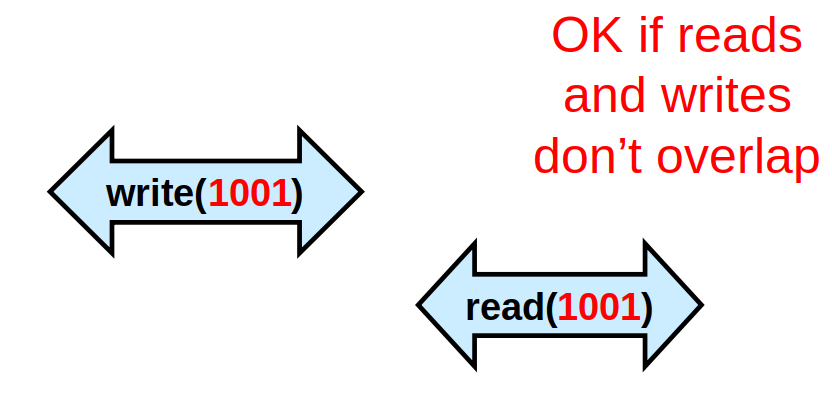
\includegraphics[width=0.5\textwidth]{./pics/safe/safe1.png}
\end{center}
}

\only<3>{
\begin{center}
  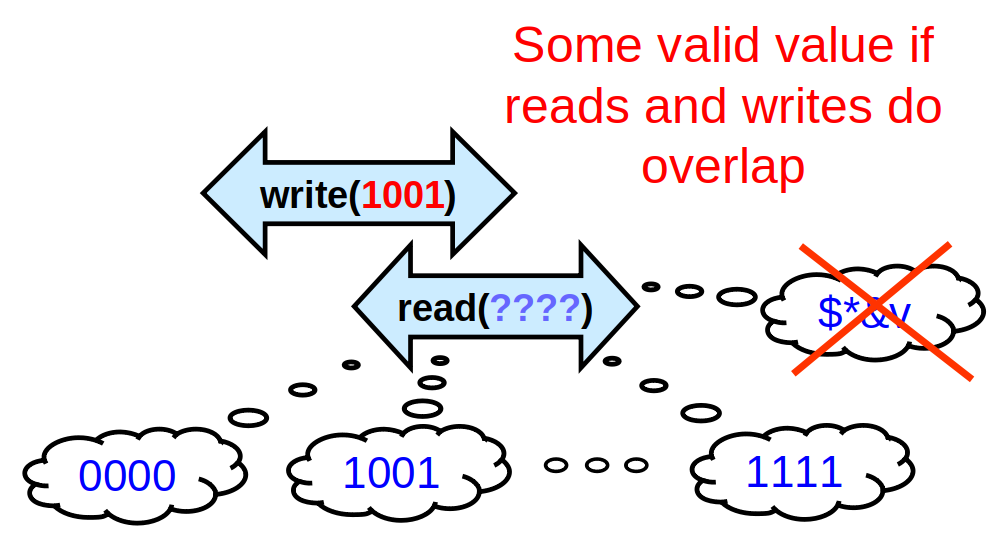
\includegraphics[width=0.5\textwidth]{./pics/safe/safe2.png}
\end{center}
}

\end{frame}

\begin{frame}[t,fragile]{Register consistency: regular register}

Regular Register:
\begin{itemize}
  \item Returns old value if no overlap (safe)
  
  \pause
  \item Old or one of new values if overlap (not arbitrary)
\end{itemize}

\pause

\only<3>{
\begin{center}
  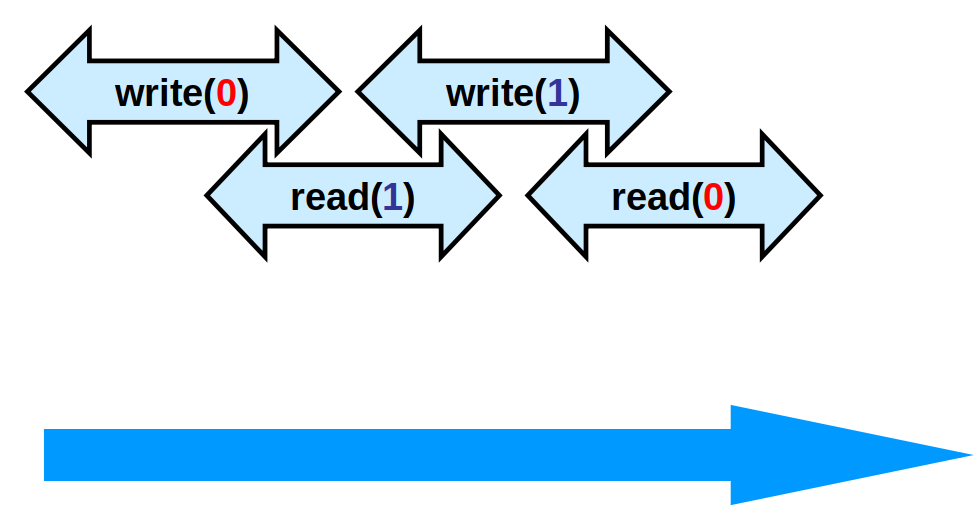
\includegraphics[width=0.5\textwidth]{./pics/regular/reg1.png}
\end{center}
}

\only<4>{
\begin{center}
  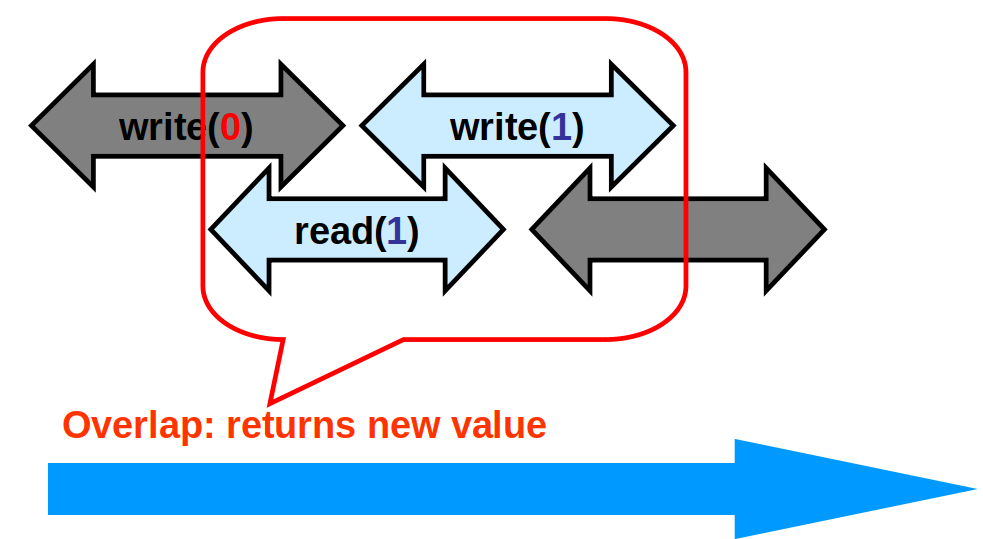
\includegraphics[width=0.5\textwidth]{./pics/regular/reg2.png}
\end{center}
}

\only<5>{
\begin{center}
  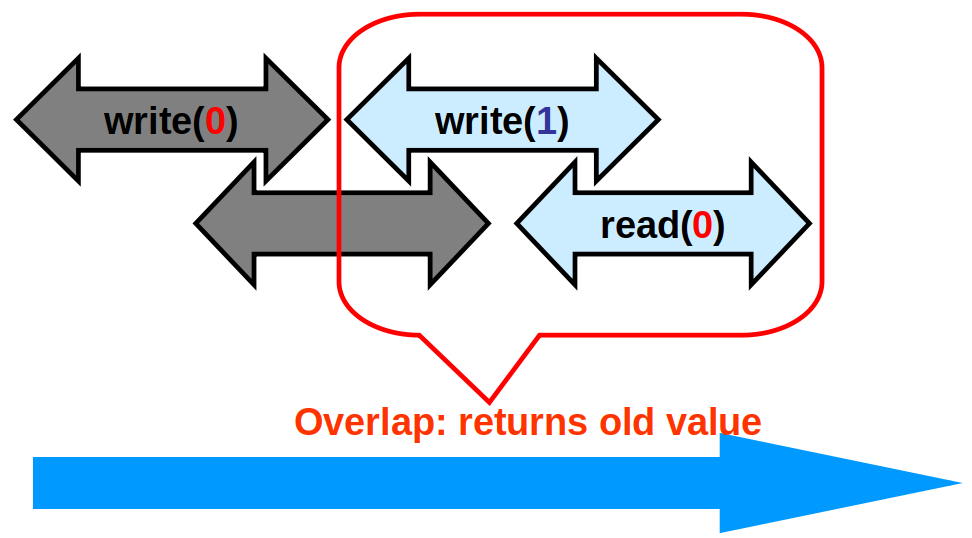
\includegraphics[width=0.5\textwidth]{./pics/regular/reg3.png}
\end{center}
}

\only<6>{
\begin{center}
  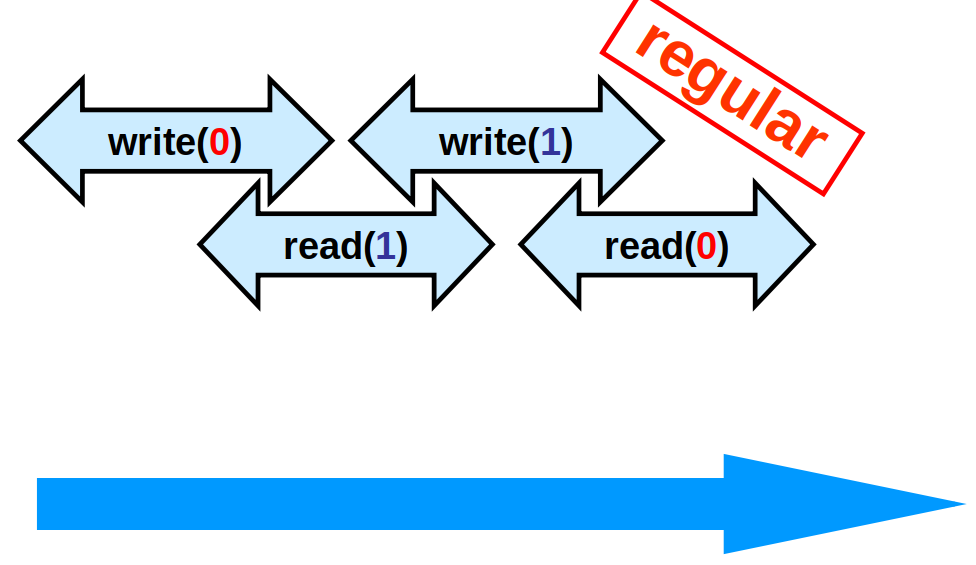
\includegraphics[width=0.5\textwidth]{./pics/regular/reg4.png}
\end{center}
}

\end{frame}

\begin{frame}{Register consistency: regular register != linearizable}

Regular Register:
\begin{itemize}
  \item Returns old value if no overlap (safe)
  \item Old or one of new values if overlap (not arbitrary)
\end{itemize}

\begin{center}
  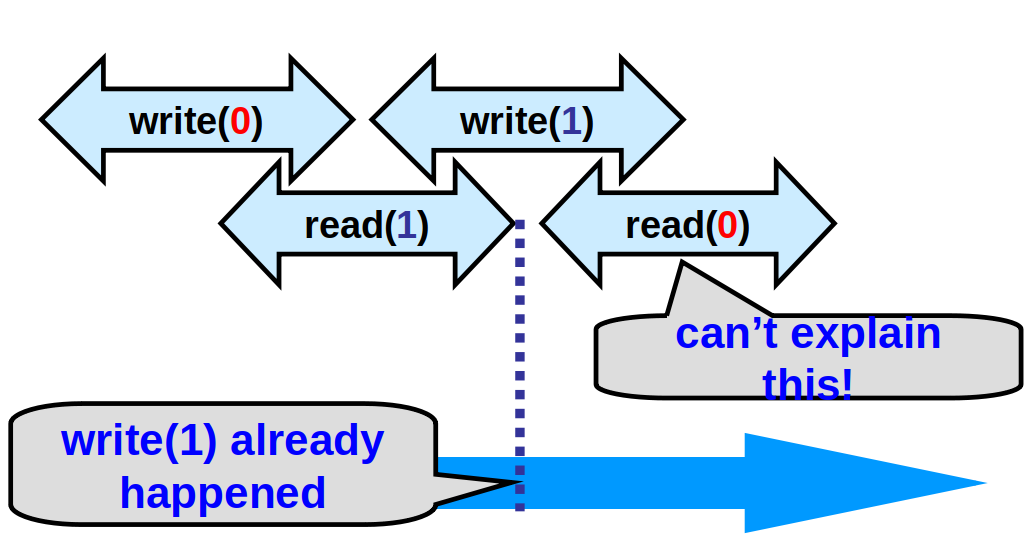
\includegraphics[width=0.5\textwidth]{./pics/regular/reg5.png}
\end{center}

\pause

\begin{center}
  \textbf{Regular != linearizable}
\end{center}

\end{frame}


\begin{frame}[t,fragile]{Register consistency: atomic register}

\begin{center}
  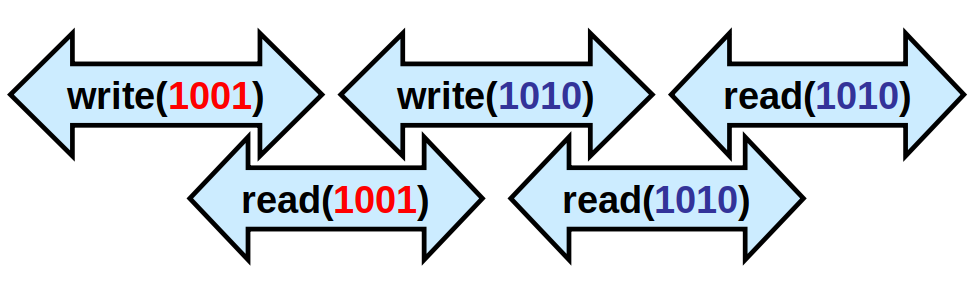
\includegraphics[width=0.5\textwidth]{./pics/atomic/atomic1.png}
\end{center}

Linearizable to sequential safe register

\end{frame}


\begin{frame}[t,fragile,noframenumbering]{Register consistency: atomic register}

\begin{center}
  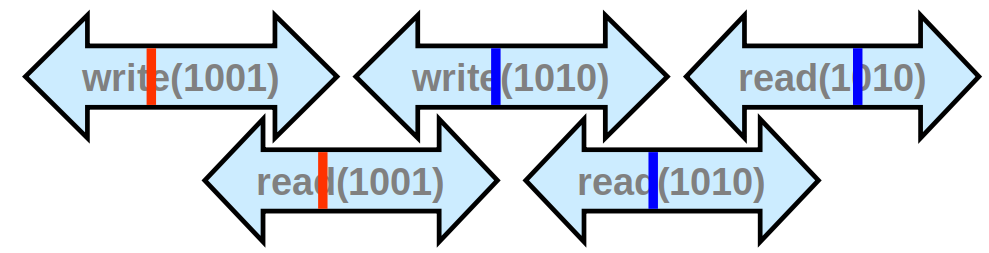
\includegraphics[width=0.5\textwidth]{./pics/atomic/atomic2.png}
\end{center}

Linearizable to sequential safe register

\end{frame}

\begin{frame}[fragile]{Register consistency: jokes to help}

\begin{itemize}
  \item Register means shared memory location

  \pause
  \item \textbf{Safe} register is quite unsafe -- generates random values under contention
  
  \pause
  \item \textbf{Regular} register exhibits irregular behaviour -- could oscillate under contention

  \pause
  \item \textbf{Atomic} register changes state somewhere inside method -- linearization point depends on execution
\end{itemize}
\end{frame}

\begin{frame}{Register space}

\begin{center}
  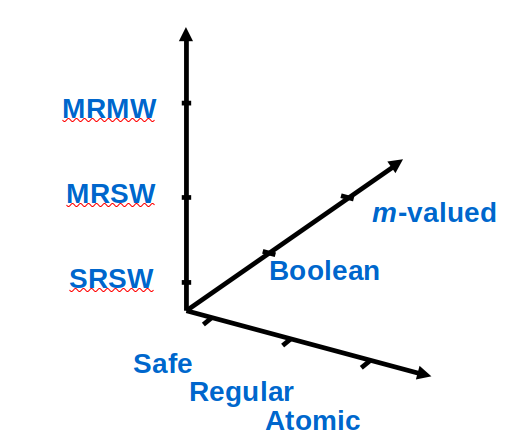
\includegraphics[width=0.5\textwidth]{./pics/space1.png}
\end{center}

\end{frame}


\begin{frame}[fragile, t]{Weakest register}

SRSW Safe Boolean register

\only<2>{
\begin{center}
  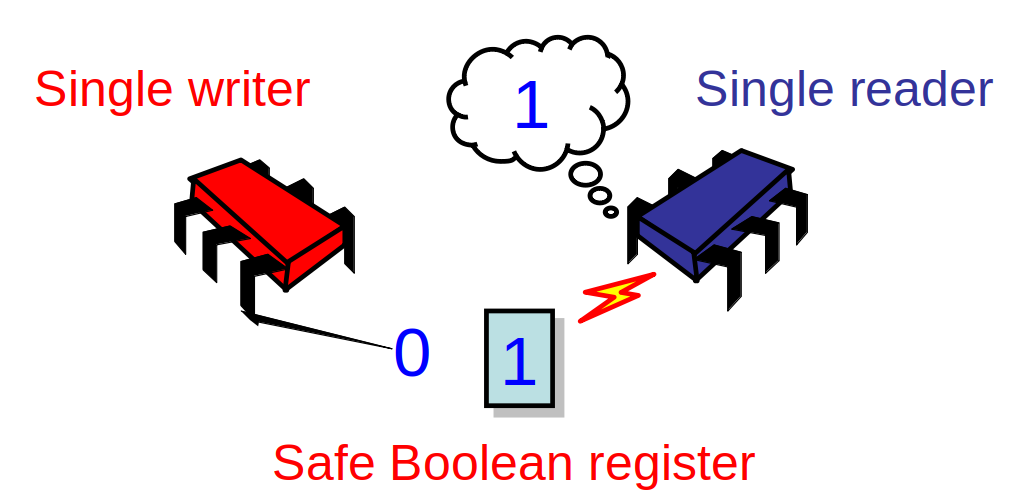
\includegraphics[width=0.5\textwidth]{./pics/weakest1.png}
\end{center}
}

\only<3>{
\begin{center}
  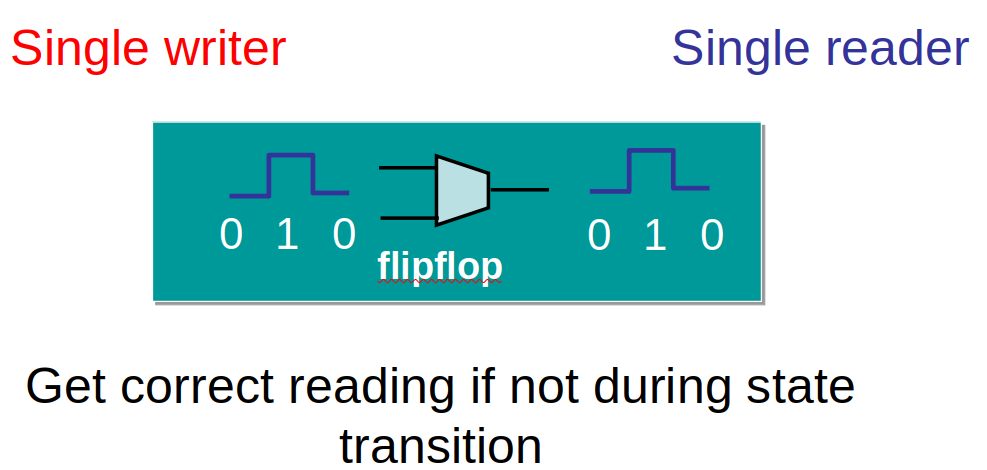
\includegraphics[width=0.5\textwidth]{./pics/weakest2.png}
\end{center}
}

\end{frame}

\begin{frame}{Spoilers}

From SRSW safe Boolean register:
\begin{itemize}
  \pause
  \item All the other registers

  \pause
  \item Mutual exclusion

  \pause
  \item Consistent and non-blocking snapshot of $N$ registers
\end{itemize}

\pause

But not everything!
\begin{itemize}
  \item Consensus hierarchy
\end{itemize}

\end{frame}

\section{Register constructions}
\showTOC

\begin{frame}{Register constructions: plan}

Not interesting to rely on mutual exclusion in register constructions
\begin{itemize}
  \item We want registers to implement mutual exclusion!
  \item It’s cheating to use mutual exclusion to implement itself!
\end{itemize}

\pause

\begin{definition}
  An object implementation is \textbf{wait-free} if every method call completes in a finite number of steps 
\end{definition} 

\pause

No mutual exclusion
\begin{itemize}
  \item Thread could halt in critical section
  \item Build mutual exclusion from registers
\end{itemize}
\end{frame}

\begin{frame}{Register constructions: plan}

From Safe SRSW Boolean to Atomic Snapshots

\begin{center}
  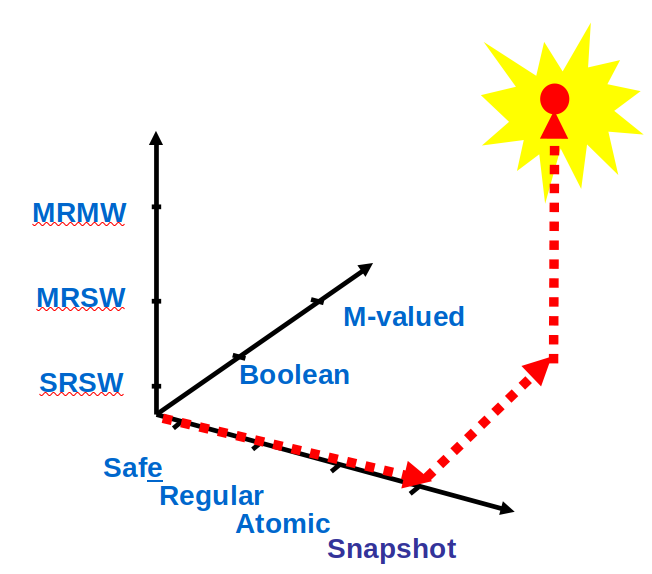
\includegraphics[width=0.4\textwidth]{./pics/space2.png}
\end{center}

\end{frame}


\begin{frame}{Register constructions: road map}

\begin{itemize}
  \item SRSW Safe Boolean
  \item MRSW Safe Boolean
  \item MRSW Regular Boolean
  \item MRSW Regular
  \item MRSW Atomic
  \item MRMW Atomic
  \item Atomic snapshot
\end{itemize}

\end{frame}


\begin{frame}[noframenumbering]{Register constructions: road map}

\begin{itemize}
  \item SRSW Safe Boolean \textbf{(1)}
  \item MRSW Safe Boolean \textbf{(2)}
  \item MRSW Regular Boolean
  \item MRSW Regular
  \item MRSW Atomic
  \item MRMW Atomic
  \item Atomic snapshot
\end{itemize}

\end{frame}

\begin{frame}[t,fragile]{Safe MRSW Boolean from Safe SRSW Boolean: notation}

\begin{minted}{java}
public class SafeBoolMRSWRegister implements Register<Boolean> {
  public boolean read() { ... }
  public void write(boolean x) { .. }
}
\end{minted}

\pause

\begin{itemize}
  \item \texttt{Safe} -- consistency
  \item Bool -- capacity
  \item MRSW -- concurrency
\end{itemize}

\end{frame}


\begin{frame}[t,fragile]{Safe MRSW Boolean from Safe SRSW Boolean: idea}

\only<1>{
\begin{center}
  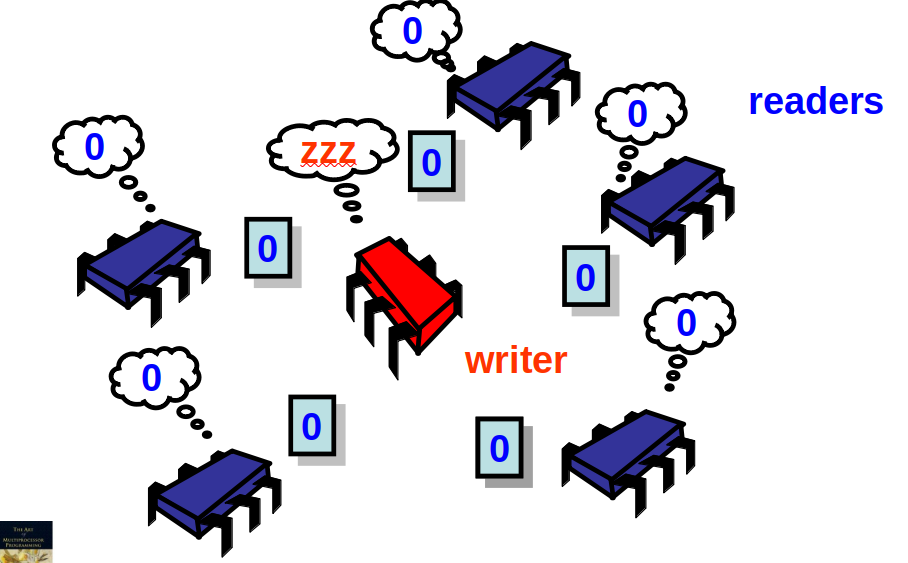
\includegraphics[width=0.5\textwidth]{./pics/c1/1.png}
\end{center}
}

\only<2>{
\begin{center}
  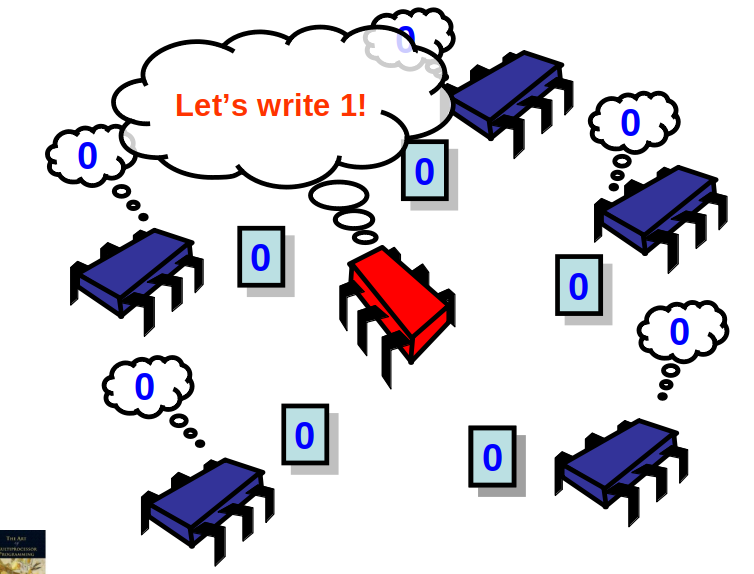
\includegraphics[width=0.5\textwidth]{./pics/c1/2.png}
\end{center}
}

\only<3>{
\begin{center}
  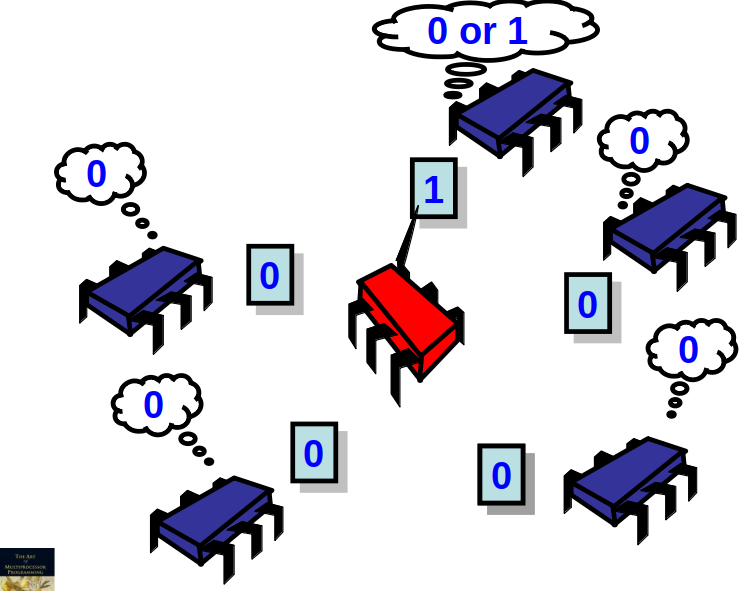
\includegraphics[width=0.5\textwidth]{./pics/c1/3.png}
\end{center}
}

\only<4>{
\begin{center}
  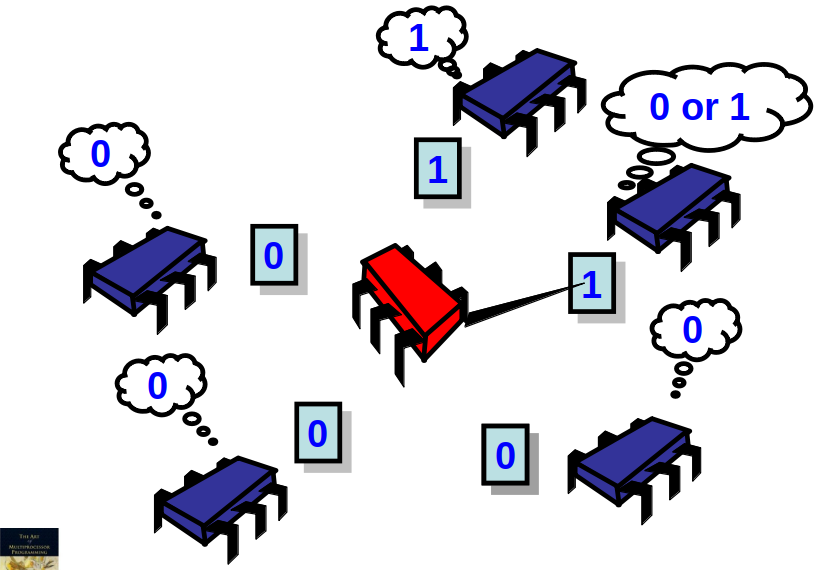
\includegraphics[width=0.5\textwidth]{./pics/c1/4.png}
\end{center}
}

\only<5>{
\begin{center}
  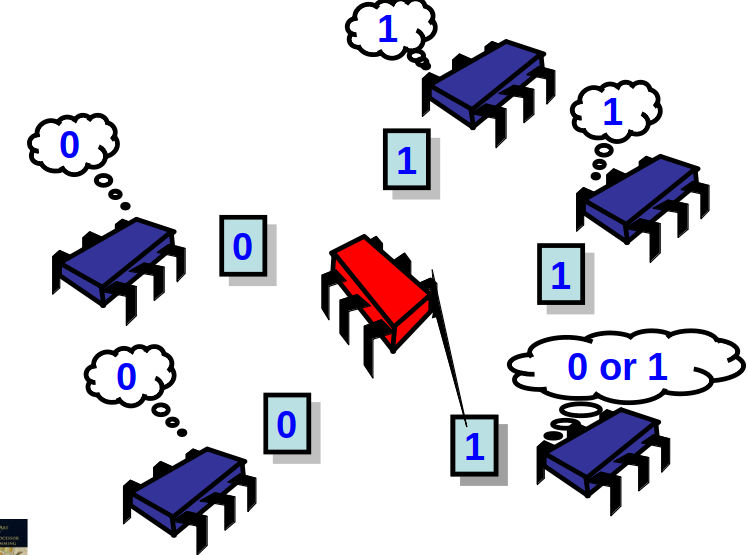
\includegraphics[width=0.5\textwidth]{./pics/c1/5.png}
\end{center}
}

\only<6>{
\begin{center}
  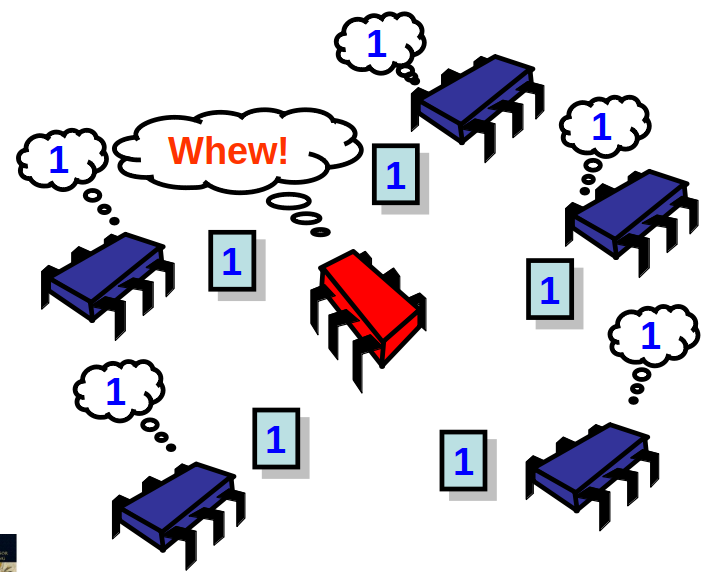
\includegraphics[width=0.5\textwidth]{./pics/c1/6.png}
\end{center}
}
\end{frame}

\begin{frame}[t,fragile]{Safe MRSW Boolean from Safe SRSW Boolean}

\begin{minted}{java}
public class SafeBoolMRSWRegister implements Register<Boolean> {
  // use weaker registers
  private SafeBoolSRSWRegister[] r = new SafeBoolSRSWRegister[N];

  public void write(boolean x) {
    for (int j = 0; j < N; j++) {
      r[j].write(x); // announce new value for every other thread
    }
  }
  public boolean read() {
    int i = ThreadID.get();
    return r[i].read(); // read own copy
  }
}
\end{minted}
\end{frame}


\begin{frame}{Register constructions: road map}

\begin{itemize}
  \item SRSW Safe Boolean 
  \item MRSW Safe Boolean \textbf{(2)}
  \item MRSW Regular Boolean \textbf{(3)}
  \item MRSW Regular
  \item MRSW Atomic
  \item MRMW Atomic
  \item Atomic snapshot
\end{itemize}

\end{frame}

\begin{frame}{Regular MRSW Boolean from Safe MRSW Boolean: idea}

\only<1>{
\begin{center}
  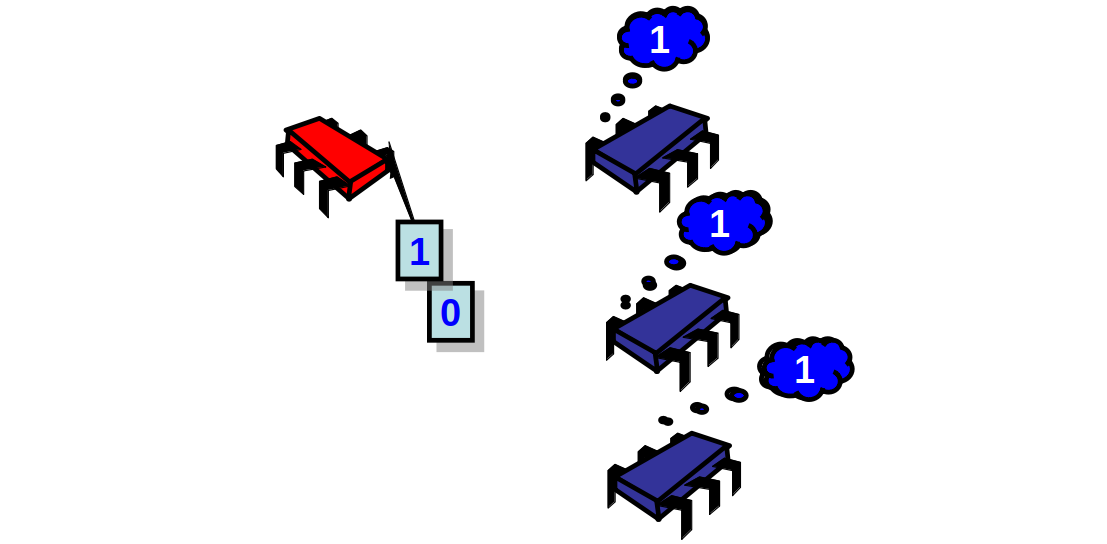
\includegraphics[width=0.5\textwidth]{./pics/c2/1.png}
\end{center}
}

\only<2>{
\begin{center}
  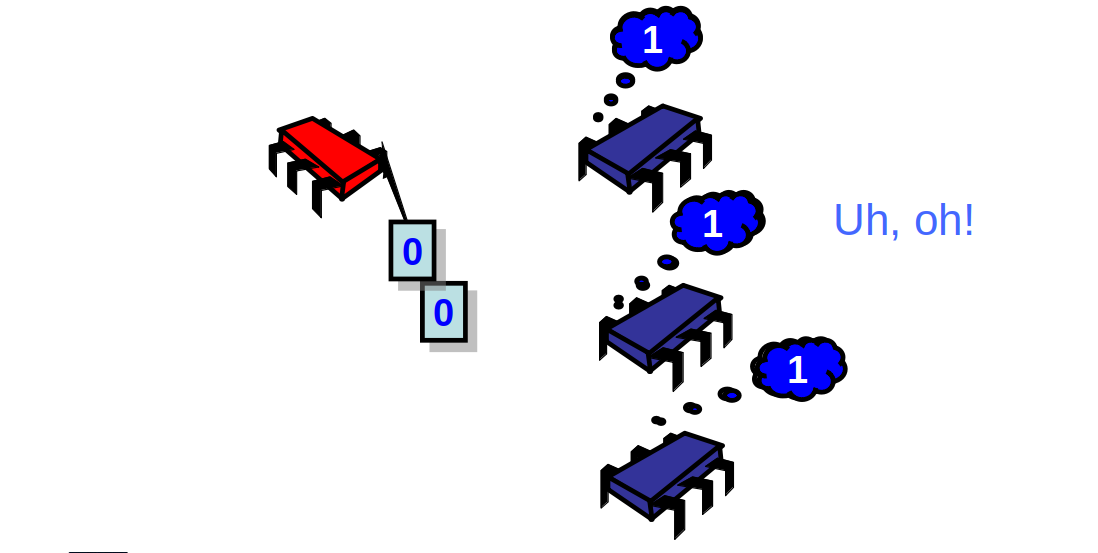
\includegraphics[width=0.5\textwidth]{./pics/c2/2.png}
\end{center}
}

\only<3>{
\begin{center}
  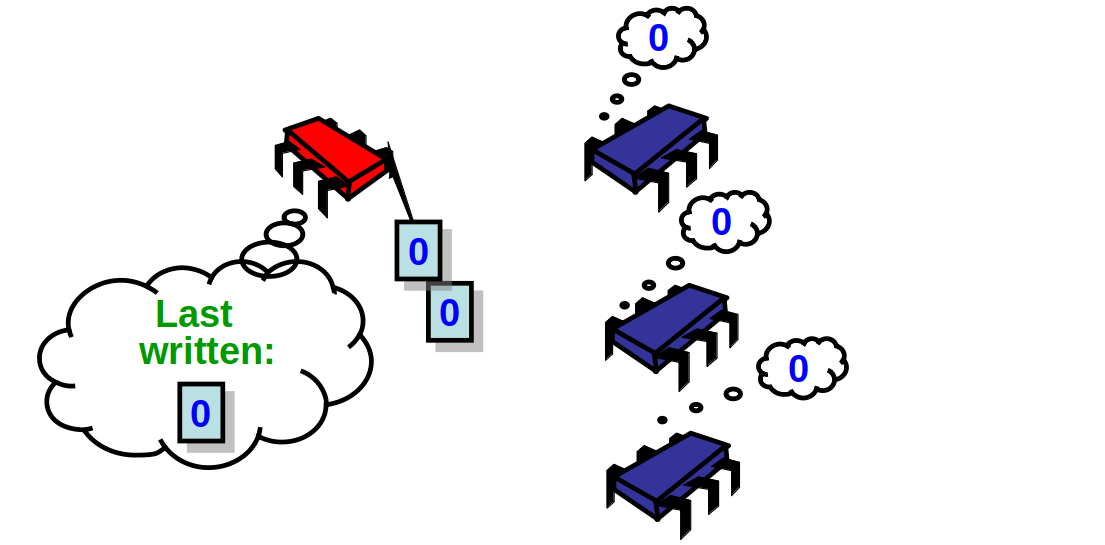
\includegraphics[width=0.5\textwidth]{./pics/c2/3.png}
\end{center}
}

\end{frame}

\begin{frame}[fragile]{Regular MRSW Boolean from Safe MRSW Boolean: idea}

\begin{minted}{java}
public class RegBoolMRSWRegister implements Register<Boolean> {
  private SafeBoolMRSWRegister value; // actual data
  private thread_local boolean old; // last bit this thread wrote
  public void write(boolean x) {
    if (old != x) {   // if new value is different from my previous write
      value.write(x); // then update
      old = x;        // remember my decision
    }
  }
  public boolean read() {
    return value.read(); // in case of overlap any result (true/false) is OK
  }
}
\end{minted}
\end{frame}


\begin{frame}{Register constructions: road map}

\begin{itemize}
  \item SRSW Safe Boolean 
  \item MRSW Safe Boolean 
  \item MRSW Regular Boolean \textbf{(3)}
  \item MRSW Regular \textbf{(4)}
  \item MRSW Atomic
  \item MRMW Atomic
  \item Atomic snapshot
\end{itemize}

\end{frame}

\begin{frame}{Representing m values}

\only<1>{
\begin{center}
  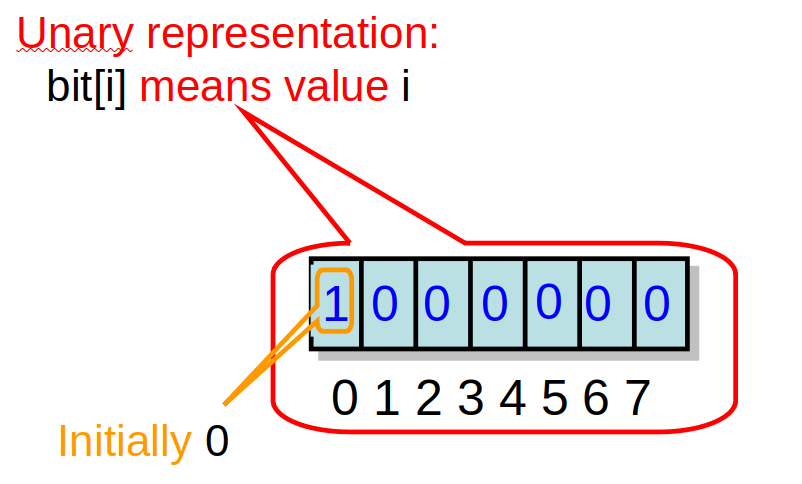
\includegraphics[width=0.5\textwidth]{./pics/unary/unary1.png}
\end{center}
}

\only<2>{
\begin{center}
  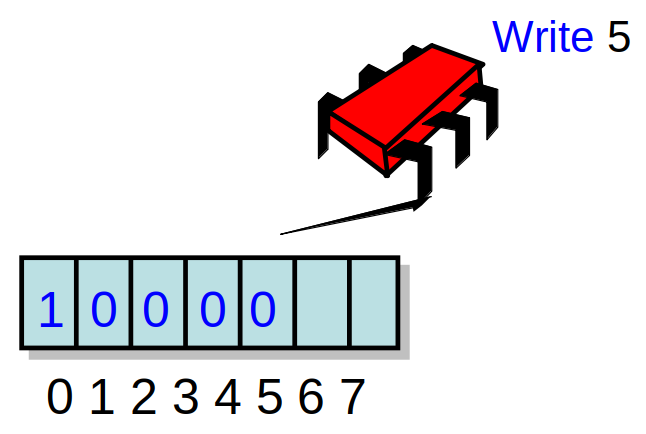
\includegraphics[width=0.5\textwidth]{./pics/unary/unary2.png}
\end{center}
}

\only<3>{
\begin{center}
  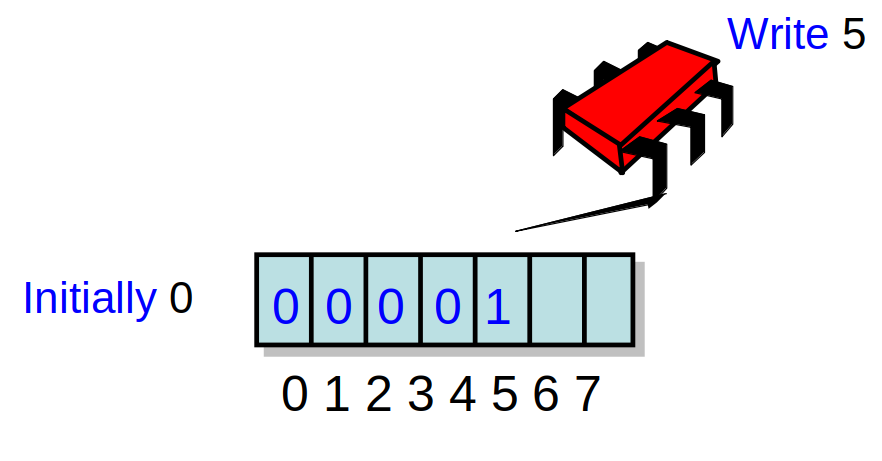
\includegraphics[width=0.5\textwidth]{./pics/unary/unary3.png}
\end{center}
}

\end{frame}

\begin{frame}[fragile]{Regular MRSW Integer from Regular MRSW Boolean}

\begin{minted}{java}
public class RegIntMRSWRegister implements Register<Integer> {
  RegBoolMRSWRegister[M] bit; // unary representation: bit[i] means value i
  public void write(int x) {
    bit[x].write(true);       // set bit x
    for (int i = x - 1; i >= 0; i--) {
      bit[i].write(false);    // clear bits from higher to lower
    }
  }
  public int read() {
    for (int i = 0; i < M; i++) { // Scan from lower to higher
      if (bit[i].read()) {        // return first bit set
        return i;
      }
    }
  }
}
\end{minted}

\end{frame}


\begin{frame}{Critical task №2: easy}

\begin{homeworkcritical}
  Prove that Regular MRSW Integer construction is correct and wait-free.

  Use Section 4.2.3 "A Regular M-Valued MRSW Register"
\end{homeworkcritical}

\end{frame}


\begin{frame}{Register constructions: road map}

\begin{itemize}
  \item SRSW Safe Boolean 
  \item MRSW Safe Boolean 
  \item MRSW Regular Boolean 
  \item MRSW Regular \textbf{(4)}
  \item MRSW Atomic \textbf{(5)}
  \item MRMW Atomic
  \item Atomic snapshot
\end{itemize}

\end{frame}


\begin{frame}[noframenumbering]{Register constructions: road map}

\begin{itemize}
  \item SRSW Safe Boolean 
  \item MRSW Safe Boolean 
  \item MRSW Regular Boolean 
  \item MRSW Regular \textbf{(4)}
  \begin{itemize}
    \item SRSW Atomic \textbf{(4.5)} \only<2->{(proof)}    
  \end{itemize}
  \item MRSW Atomic \textbf{(5)} \only<3->{(idea)}
  \item MRMW Atomic
  \item Atomic snapshot
\end{itemize}

\end{frame}


\begin{frame}[noframenumbering]{Register constructions: road map}

\begin{itemize}
  \item SRSW Safe Boolean 
  \item MRSW Safe Boolean 
  \item MRSW Regular Boolean 
  \item MRSW Regular \textbf{(4)}
  \begin{itemize}
    \item SRSW Atomic \textbf{(4.5)} (proof)
  \end{itemize}
  \item MRSW Atomic
  \item MRMW Atomic
  \item Atomic snapshot
\end{itemize}

\end{frame}

\begin{frame}[fragile]{Atomic SRSW from Regular SRSW: problem}

\only<1>{
\begin{center}
  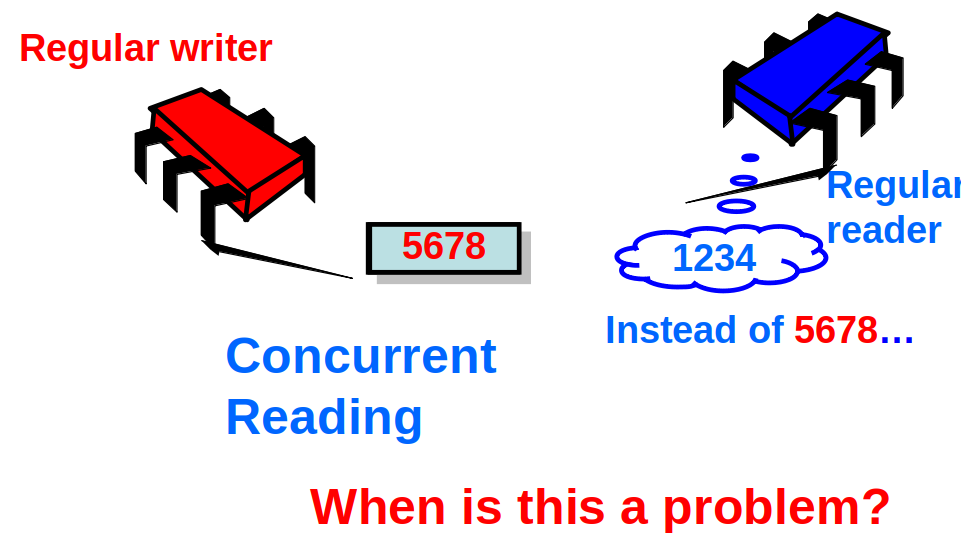
\includegraphics[width=0.5\textwidth]{./pics/sr-atomic/sr1.png}
\end{center}
}

\only<2>{
\begin{center}
  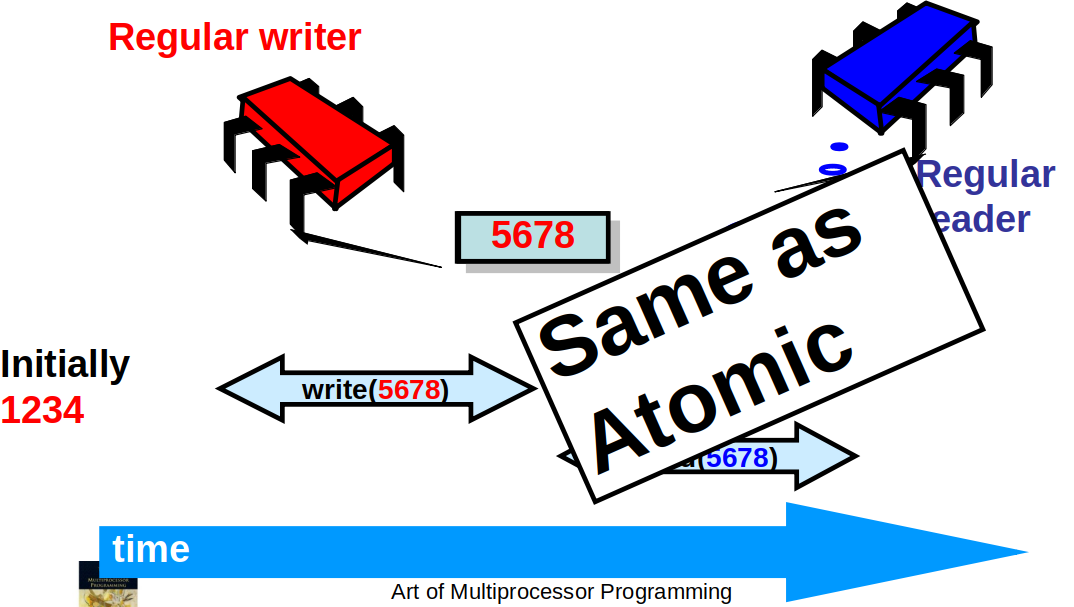
\includegraphics[width=0.5\textwidth]{./pics/sr-atomic/sr2.png}
\end{center}
}

\only<3>{
\begin{center}
  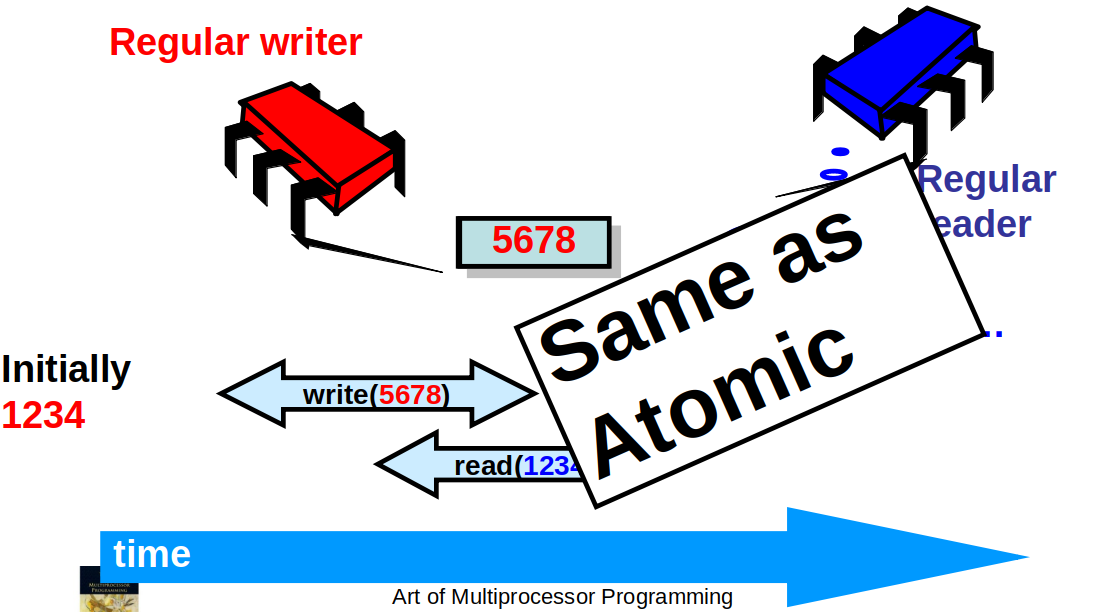
\includegraphics[width=0.5\textwidth]{./pics/sr-atomic/sr3.png}
\end{center}
}

\only<4>{
\begin{center}
  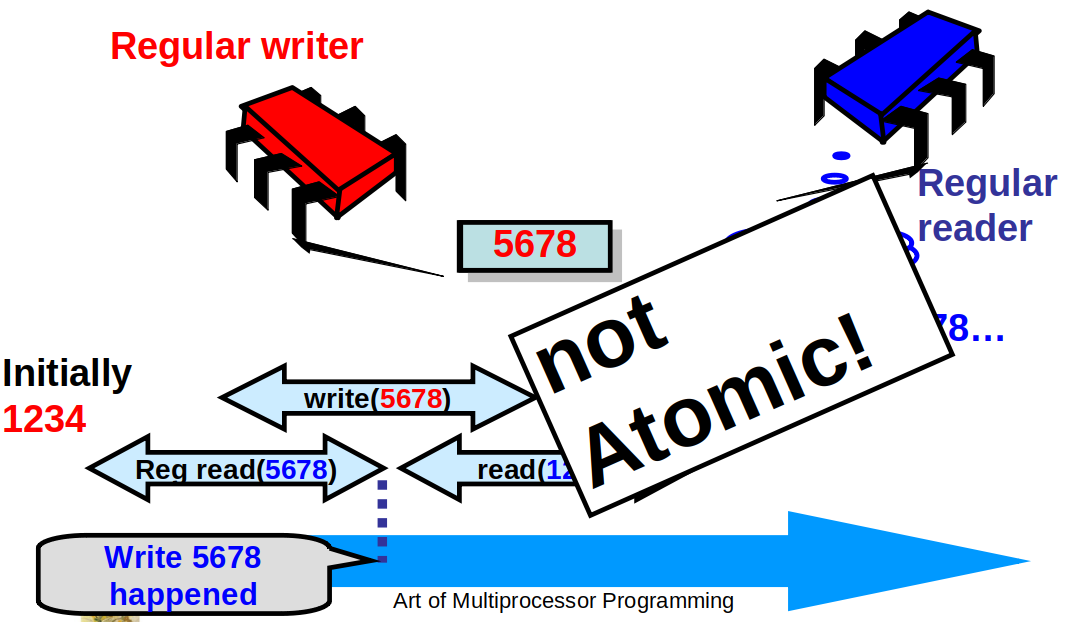
\includegraphics[width=0.5\textwidth]{./pics/sr-atomic/sr4.png}
\end{center}
}
\end{frame}


\begin{frame}[fragile]{Atomic SRSW from Regular SRSW: timestamped values}

\only<1>{
\begin{center}
  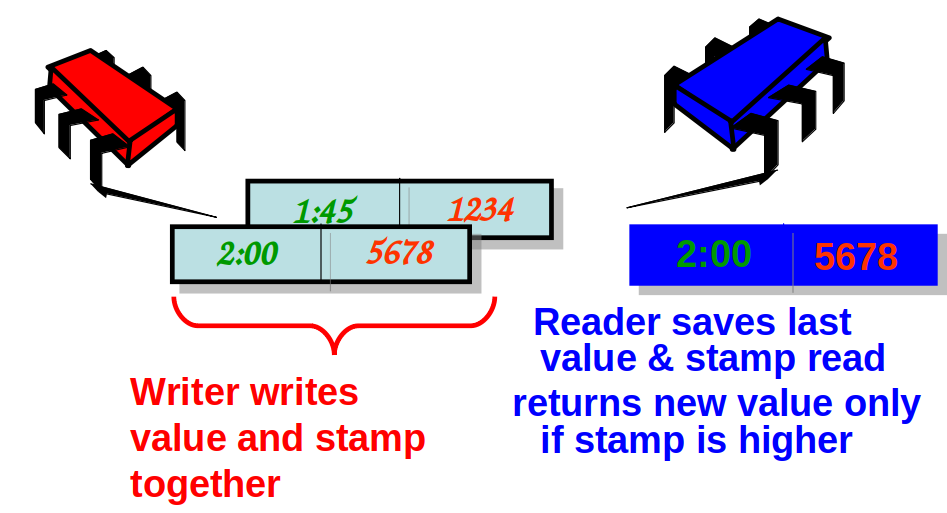
\includegraphics[width=0.5\textwidth]{./pics/stamp/stamp1.png}
\end{center}
}

\only<2->{
\begin{center}
  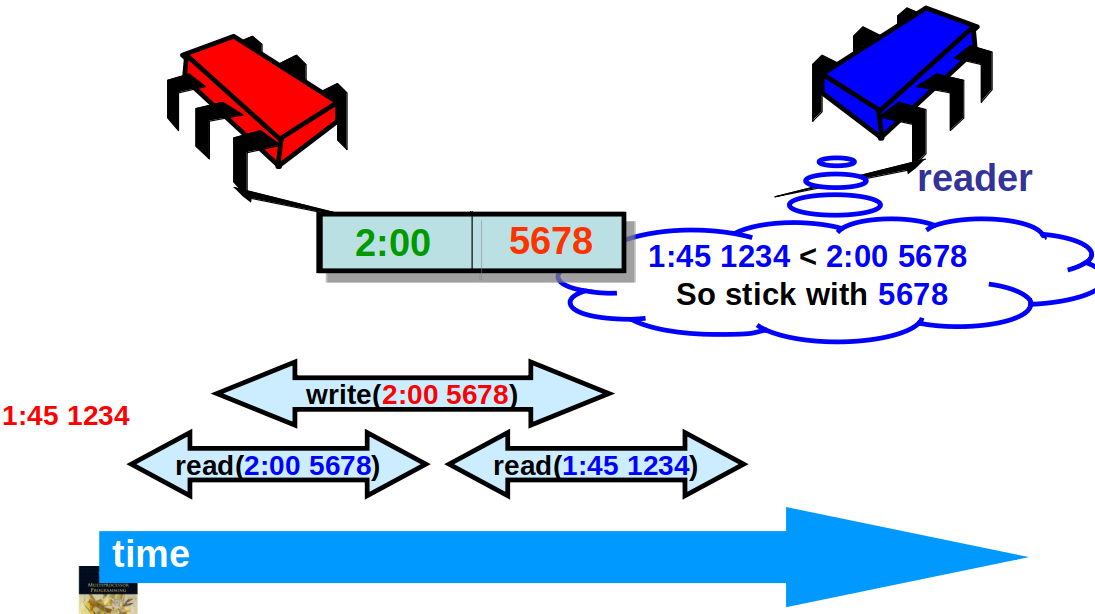
\includegraphics[width=0.5\textwidth]{./pics/stamp/stamp2.png}
\end{center}
}

\only<3->{
\begin{center}
  \textbf{Same as atomic}
\end{center}
}

\end{frame}


\begin{frame}{Timestamped values: clock problem}

How different threads coordinate "current time"?
\begin{itemize}
  \pause
  \item They need some kind of consistent global clock
  \pause
  \item Mutual exclusion?
\end{itemize}

\pause
We cannot "cheat" \ by using real clock time. 

\pause
In previous construction we were building \textbf{single-writer single-reader} register
\begin{itemize}
  \pause
  \item Writer was timestamping data

  \pause
  \item Reader used stamps to track "latest" \ updates
\end{itemize}

\pause
Clock == writer-specific integer counter

\pause
\textbf{Beware:} ensure you understand what is called "timestamp" \ in the following proofs

\end{frame}


\begin{frame}{Register constructions: road map}

\begin{itemize}
  \item SRSW Safe Boolean 
  \item MRSW Safe Boolean 
  \item MRSW Regular Boolean 
  \item MRSW Regular
  \begin{itemize}
    \item SRSW Atomic \textbf{(4.5)}
  \end{itemize}
  \item MRSW Atomic \textbf{(5)} \only<2->{(idea)}
  \item MRMW Atomic
  \item Atomic snapshot
\end{itemize}
\end{frame}


\begin{frame}[fragile]{Atomic MRSW from Atomic SRSW: naive idea}

\only<1>{
\begin{center}
  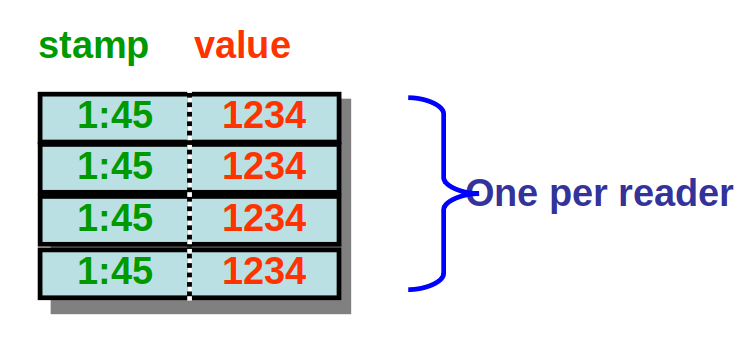
\includegraphics[width=0.5\textwidth]{./pics/mr-atomic/mr1.png}
\end{center}
}

\only<2>{
\begin{center}
  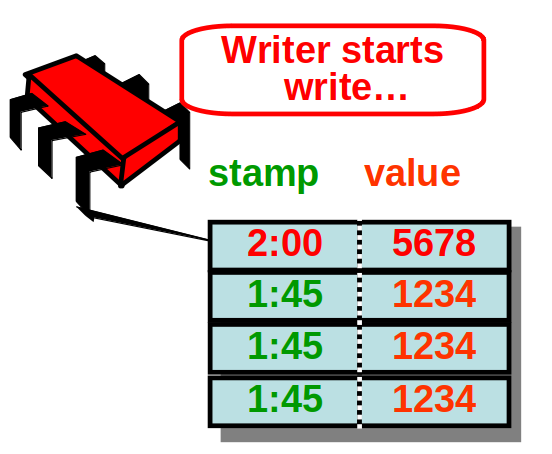
\includegraphics[width=0.5\textwidth]{./pics/mr-atomic/mr2.png}
\end{center}
}

\end{frame}


\begin{frame}[fragile]{Atomic MRSW from Atomic SRSW: naive idea does not work}

\begin{center}
  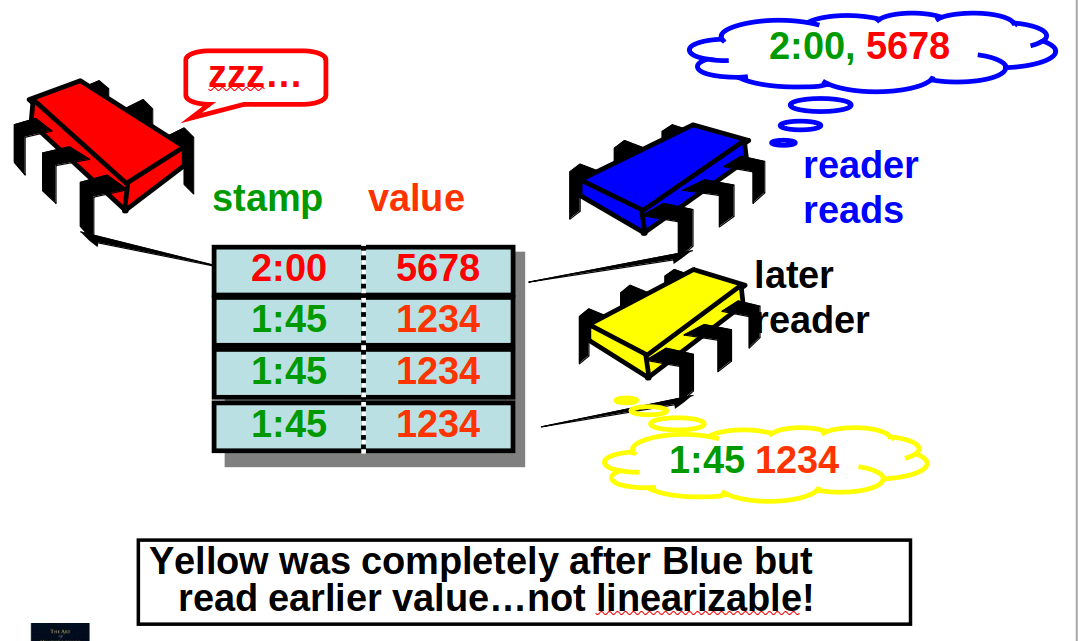
\includegraphics[width=0.5\textwidth]{./pics/mr-atomic/mr3.png}
\end{center}

\end{frame}


\begin{frame}[fragile]{Atomic MRSW from Atomic SRSW: multi-reader table}

\only<1>{
\begin{center}
  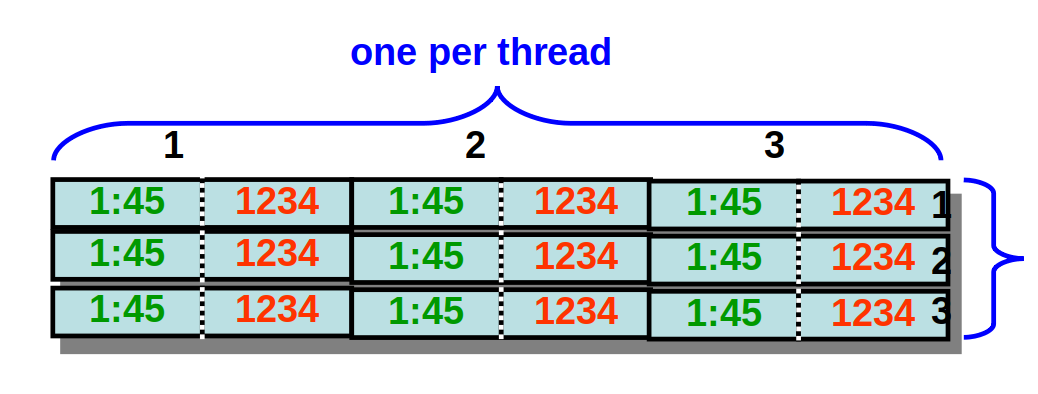
\includegraphics[width=0.5\textwidth]{./pics/mr-atomic/mr4.png}
\end{center}
}

\only<2>{
\begin{center}
  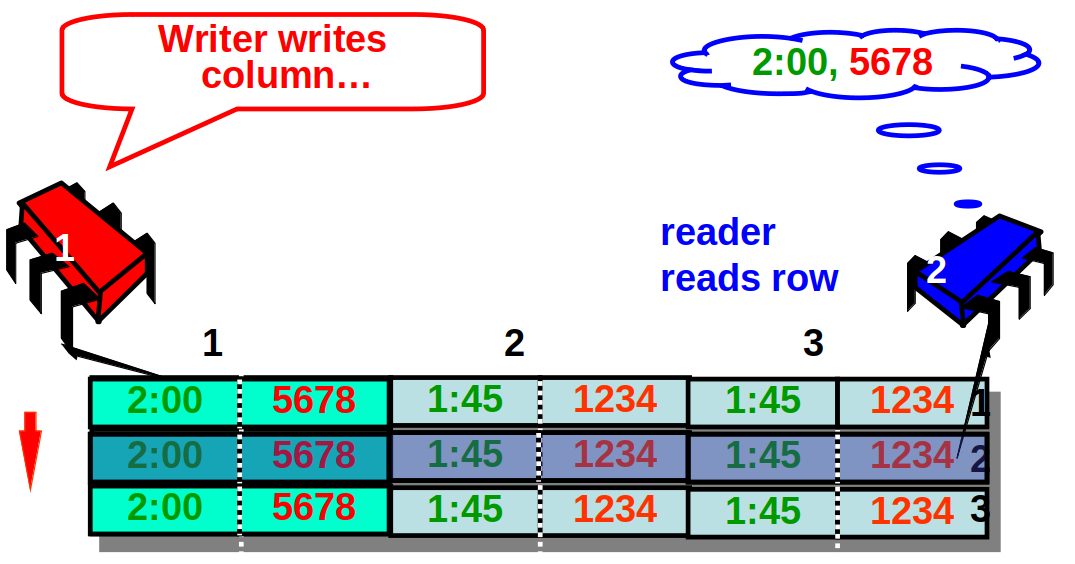
\includegraphics[width=0.5\textwidth]{./pics/mr-atomic/mr5.png}
\end{center}
}

\only<3>{
\begin{center}
  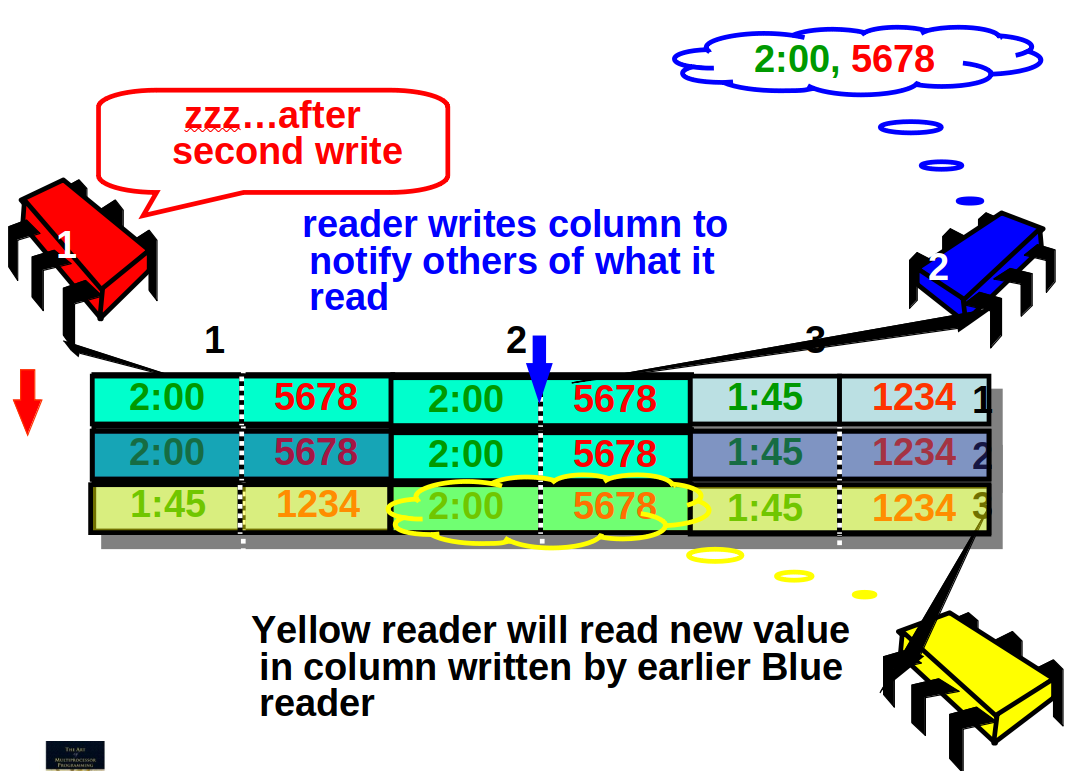
\includegraphics[width=0.5\textwidth]{./pics/mr-atomic/mr6.png}
\end{center}
}
\end{frame}

\begin{frame}[t,fragile]{Atomic MRSW from Atomic SRSW: summary}

In order to achieve high level of
\begin{itemize}
  \item consistency (linearizable)
  \item concurrency (multi-reader) 
  \item progress condition (wait-freedom)
\end{itemize}

\end{frame}


\begin{frame}[t,fragile,noframenumbering]{Atomic MRSW from Atomic SRSW: summary}

In order to achieve high level of
\begin{itemize}
  \item consistency (linearizable), concurrency (multi-reader), progress condition (wait-freedom)
\end{itemize}

\pause
we used complicated algorithm with non-obvious design solutions
\pause
\begin{itemize}
  \item Timestamping of values with writer-local clock
  \item Readers \textbf{write} values into auxiliary data structures
  \item Single high-level operation (atomic read or write) requires $N$ low-level steps (update of thread-specific regular registers)
\end{itemize}


\end{frame}

\begin{frame}[t,fragile,noframenumbering]{Atomic MRSW from Atomic SRSW: summary}

In order to achieve high level of
\begin{itemize}
  \item consistency (linearizable), concurrency (multi-reader), progress condition (wait-freedom)
\end{itemize}

we used complicated algorithm with non-obvious design solutions
\begin{itemize}
  \item Timestamping, Readers cooperate with writers, Decomposition
\end{itemize}

\pause
which was hard to prove
\pause
\begin{itemize}
  \item Safe register is unsafe and counter-intuitive
  \item Regular register oscillate under contention
  \item Atomic register has "floating" \ linearization points
\end{itemize}

\pause
but beneficial
\pause
\begin{itemize}
  \item Any algorithm based on atomic registers could be implemented via safe SRSW boolean registers
  \item Every register construction is wait-free and does not depend on scheduler
\end{itemize}

\end{frame}


\begin{frame}{Register constructions: road map}

\begin{itemize}
  \item SRSW Safe Boolean 
  \item MRSW Safe Boolean 
  \item MRSW Regular Boolean 
  \item MRSW Regular
  \begin{itemize}
    \item SRSW Atomic     
  \end{itemize}
  \item MRSW Atomic \textbf{(5)}
  \item MRMW Atomic \textbf{(6)} \only<2->{(optional homework)}
  \item Atomic snapshot
\end{itemize}
\end{frame}

\begin{frame}[t,fragile]{Atomic MRMW from Atomic MRSW: optional homework}

Optional homework: slides 95-103 from \texttt{chapter\_04.ppt}

Optional homework: Section 4.2.6 "An Atomic MRMW Register" \ (pages 85-87)

Key insights: 
\begin{itemize}
  \item sort events by lexicographic order and prove it is consistent with \textit{precedence}
\end{itemize}

\end{frame}

\section{Atomic snapshots}
\showTOC

\begin{frame}{Atomic snapshot}

\begin{center}
  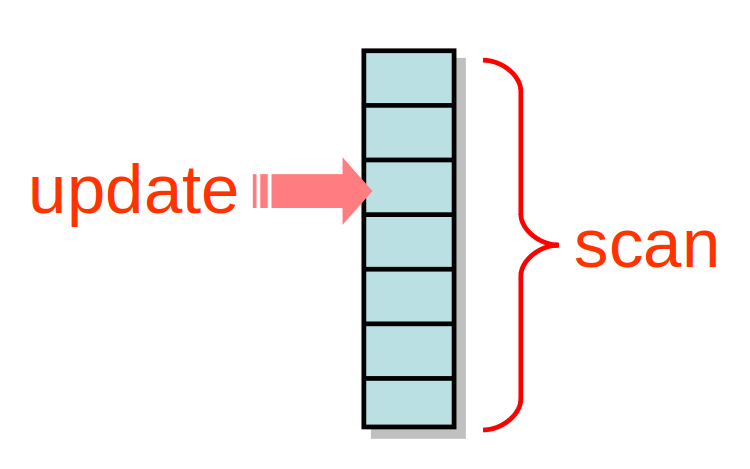
\includegraphics[width=0.5\textwidth]{./pics/snapshot1.png}
\end{center}

\end{frame}


\begin{frame}[fragile]{Atomic snapshot}

Array of MRSW atomic registers (1 register per thread)
\begin{itemize}
  \item Take instantaneous snapshot of all
  \item Generalizes to MRMW registers
\end{itemize}

\pause

\begin{minted}{java}
interface Snapshot<T> {
  // Thread.currentThread writes `v` to its own register (arr[Thread.id] = v)
  public void update(T v);
  // Instantaneous snapshot of all threads’ registers (return copy(arr))
  public T[] scan();
}
\end{minted}

\pause

Collect
\begin{itemize}
  \item Read values one at a time
\end{itemize}

Problem
\begin{itemize}
  \item Incompatible concurrent collects
  \item Result not linearizable
\end{itemize}

\end{frame}


\begin{frame}{Clean collect}

Clean Collect
\begin{itemize}
  \item Collect during which nothing changed
\end{itemize}

\pause

Challenge
\begin{itemize}
  \item Can we make it happen?
  \item Can we detect it?
\end{itemize}

\pause
Simple snapshot:
\begin{itemize}
  \item \only<1-3>{Put increasing labels on each entry} \only<4->{\textbf{Put increasing labels on each entry (why?)}}
  \item Collect twice
  \item If both agree -- we are done
  \item Otherwise -- try again
\end{itemize}

\pause
\pause
Problem: Scanner might not be collecting a snapshot!

\end{frame}


\begin{frame}[fragile]{Clean collect: must use labels}

\only<1>{
\begin{center}
  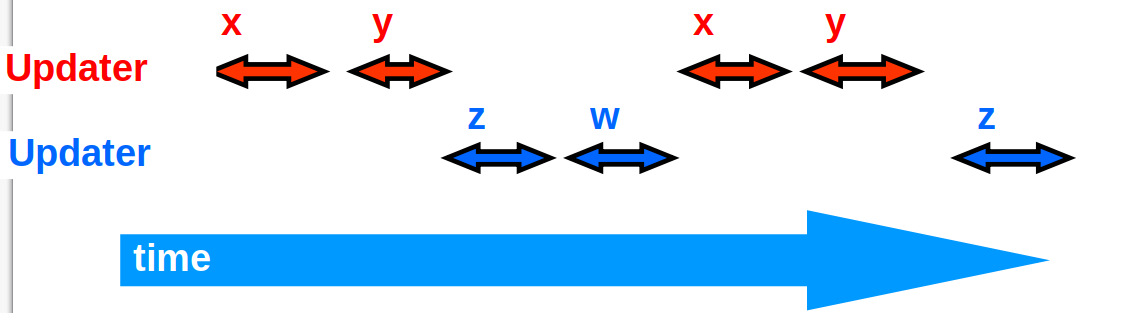
\includegraphics[width=0.5\textwidth]{./pics/snap-label/lbl1.png}
\end{center}
}

\only<2>{
\begin{center}
  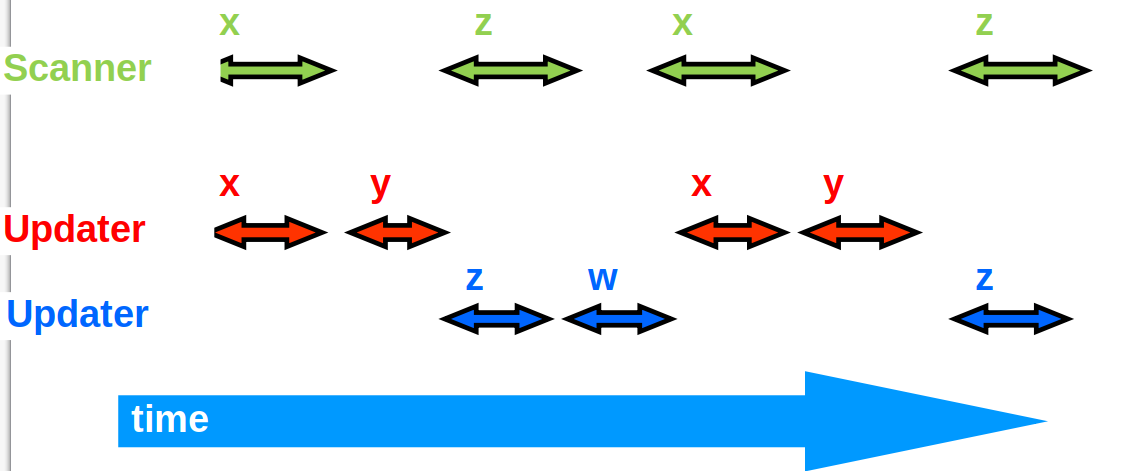
\includegraphics[width=0.5\textwidth]{./pics/snap-label/lbl2.png}
\end{center}
}

\only<3>{
\begin{center}
  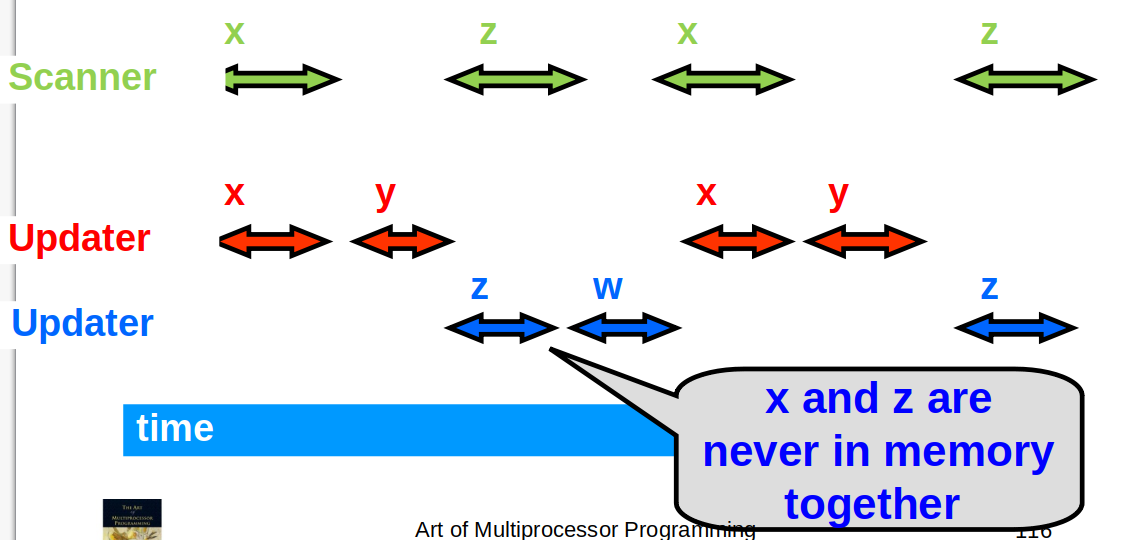
\includegraphics[width=0.5\textwidth]{./pics/snap-label/lbl3.png}
\end{center}
}

\only<4>{
\begin{center}
  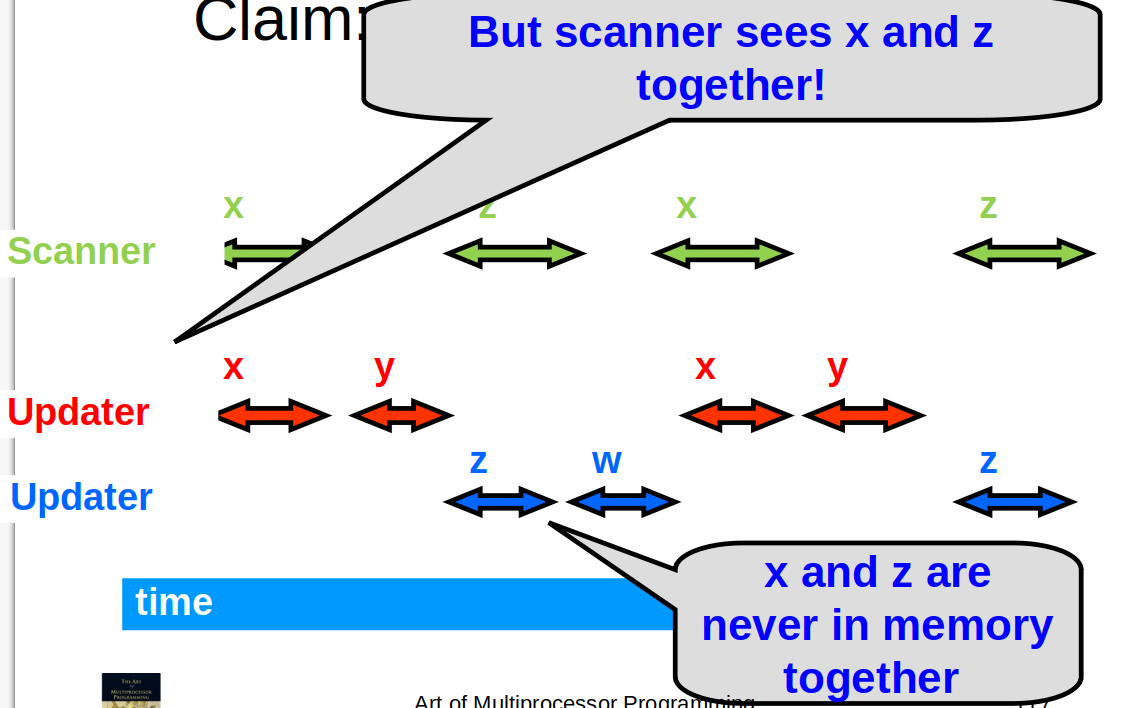
\includegraphics[width=0.5\textwidth]{./pics/snap-label/lbl4.png}
\end{center}
}

\only<5>{
\begin{center}
  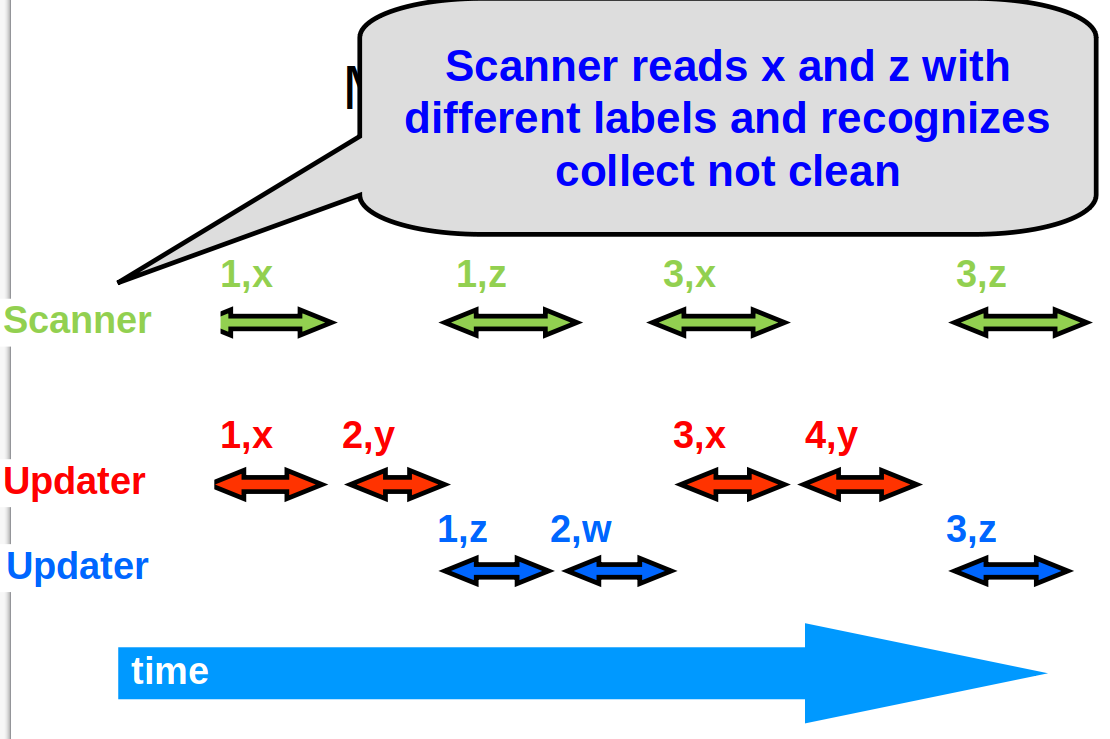
\includegraphics[width=0.5\textwidth]{./pics/snap-label/lbl5.png}
\end{center}
}
\end{frame}


\begin{frame}[fragile]{ABA: first encounter}

We had a subtle concurrent problem:
\begin{itemize}
 \item Thread 1 reads some data (''current state of system'', e.g. \texttt{queue.length == 2}), denote \textbf{A}
 \item Thread 2 changes system state to \textbf{B} (e.g. \texttt{queue.enq})
 \item Thread 3 changes system state back to \textbf{A} (e.g. \texttt{queue.deq})
 \item Thread 1 reads system state again
\end{itemize}

\pause

Thread 1 thinks "nothing happened with the system" \ (e.g. no new data arrived) which is \textbf{incorrect}.

\pause

This is called ABA problem. One of the most complicated issues with non-blocking algorithms.

\pause

Timestamping helps to solve it. \pause But what if your timestamp (\texttt{int} counter) overflow and wrap? 

\pause
"The Art of Multiprocessor Programming" \ section 2.7 "Bounded Timestamps" \pause

... or just use \texttt{long} counters ;)

\end{frame}


\begin{frame}[fragile]{Simple snapshot}

\begin{minted}{java}
private AtomicMRSWRegister[] register; // reg[i] belongs to i-th Thread
public void update(T value) {
  var i = ThreadID.get(); var oldValue = register[i].read();  
  register[i].write(new LabeledValue(oldValue.label + 1, value)); 
}
private LabeledValue[] collect() {
  var copy = new LabeledValue[n];
  for (int j = 0; j < n; j++) copy[j] = register[j].read();
  return copy; 
}
public T[] scan(){ var oldCopy = collect();
  while (true) {   var newCopy = collect(); // <-----------------------------+
                   if (equals(oldCopy, newCopy)) return getValues(newCopy);//|
                   oldCopy = newCopy; // ------------------------------------+    
  }}
\end{minted}
\end{frame}


\begin{frame}[fragile]{Simple snapshot}

\begin{itemize}
  \item Linearizable
  \item Update is wait-free
  \begin{itemize}
    \item No unbounded loops
  \end{itemize}
  \item But Scan can starve \only<2->{(\textbf{Obstruction-free})}
  \begin{itemize}
    \item If interrupted by concurrent update
  \end{itemize}
\end{itemize}

\end{frame}


\begin{frame}[fragile]{Critical task №2: medium}

\begin{homeworkcritical}
  \begin{itemize}
    \item Finish "Easy" \ level.
    \item  Prove that "Simple snapshot" \ algorithm is correct, wait-free for \texttt{update()} and obstruction-free for \texttt{scan()}.
           Use Section 4.3.1 "An Obstruction-Free Snapshot".
    \item \textbf{Note:} algorithm uses stamped values, be ready to explain how it works in wait-free setting
  \end{itemize}
\end{homeworkcritical}

\end{frame}


\begin{frame}[fragile]{Critical task №2: hard}

\begin{homeworkcritical}
  \begin{itemize}
    \item Finish "Medium" \ level.    
    \item Solve exercise 41 from Section 4.5.
  \end{itemize}
\end{homeworkcritical}
\end{frame}

\begin{frame}[fragile,noframenumbering]{Critical task №2: hard}

\textbf{Exercise 41}. There are $n$ processors $P_0$, ... , $P_{n-1}$ arranged in a ring, where $P_i$ can send messages only to $P_{i+1 \ mod \ n}$.
Messages are delivered in FIFO order along each link. Each processor keeps a copy of the shared register. To read a register, the processor reads the copy in its local memory.

\begin{itemize}
  \item A processor $P_i$ starts a \texttt{write()} call of value $v$ to register $x$ by sending the message \ \ \ \ \ \ \ \texttt{“$P_i$: write v to x”} to $P_{i+1 \ mod \ n}$.
  \item If $P_i$ receives a message \texttt{“$P_j$: write v to x”} for $i \neq j$, then it writes $v$ to its local copy of $x$, and forwards the message to $P_{i+1 \ mod\  n}$.
  \item If $P_i$ receives a message \texttt{“$P_i$: write v to x”} then it writes $v$ to its local copy of $x$, and discards the message. The \texttt{write()} call is now complete.
\end{itemize}

Give a short justification or counterexample.
If \texttt{write()} calls never overlap,
\begin{itemize}
  \item Is this register implementation regular?
  \item Is it atomic?
\end{itemize}

If multiple processors call \texttt{write()},
\begin{itemize}
  \item Is this register implementation safe?
\end{itemize}


\end{frame}

\begin{frame}{Atomic snapshot: wait free}

We need progress even if other threads update data
\begin{itemize}
  \pause
  \item Every scanner does scan (as before)
  \pause
  \item Every updater does scan  (\textit{helping hand})
  \pause
  \item In case of conflicts scanner could reuse scan from updater
\end{itemize}
\pause
Good luck to prove
\begin{itemize}
  \item Reused value is consistent (resulting snapshot is linearizable)
  \item Appropriate reused value always exists (wait-freedom for every concurrent scenario)
  \item Stealing of value is correct
\end{itemize}

\pause
Optional homework: Section 4.3.2 "A Wait-Free Snapshot" \  and Section 4.3.3 "Correctness Arguments" \ (pages 88-93)

\end{frame}


\begin{frame}{Register constructions: summary}

Safe Single-Reader Single-Writer Boolean register could
\begin{itemize}
  \item implement other registers, up to Atomic MRMW Integer registers
  \item provide a consistent atomic snapshot of $N$ registers
\end{itemize}
using wait-free algorithms

\pause
What is the next step to attempt with read-write registers? 
\pause
\begin{itemize}
  \item Snapshot means
  \begin{itemize}
    \item Write any one array element
    \item Read multiple array elements
  \end{itemize}
  \pause
  \item What about atomic writes to multiple locations?
\end{itemize}
\end{frame}

\section{Consensus number}
\showTOC

\begin{frame}{Motivation}

Why do we use mutual exclusion or other communication protocol?

\pause

\begin{itemize}
  \item For thread coordination
  \pause
  \item Ensure system evolves according to some rules
  \pause
  \item Threads decide what to do together
\end{itemize}

\end{frame}


\begin{frame}{Each thread has private input}
\begin{center}
  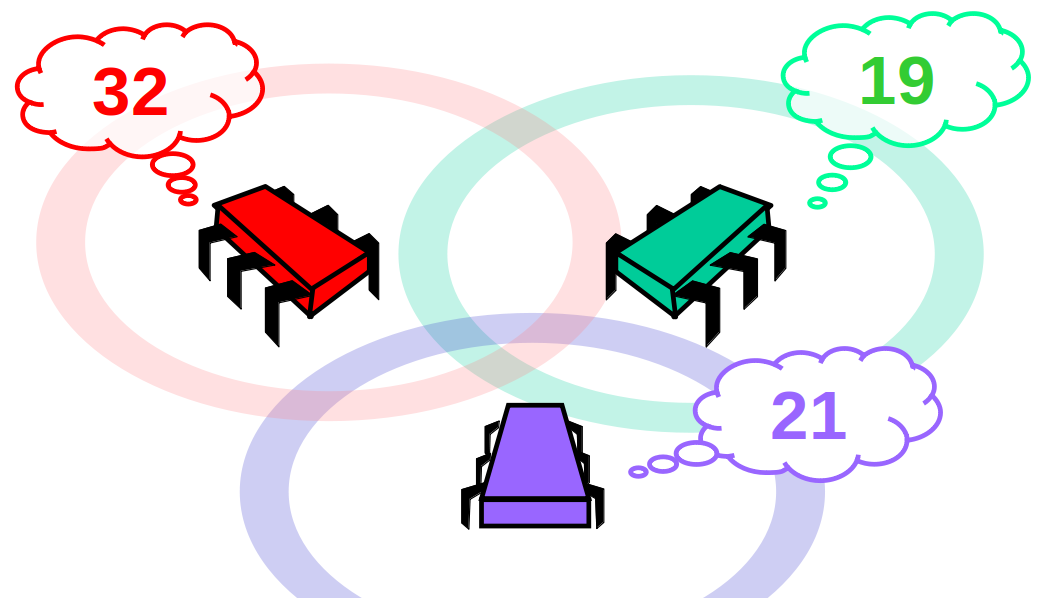
\includegraphics[width=0.5\textwidth]{./pics/consensus/cons1.png}
\end{center}
\end{frame}

\begin{frame}[noframenumbering]{They communicate}

\begin{center}
  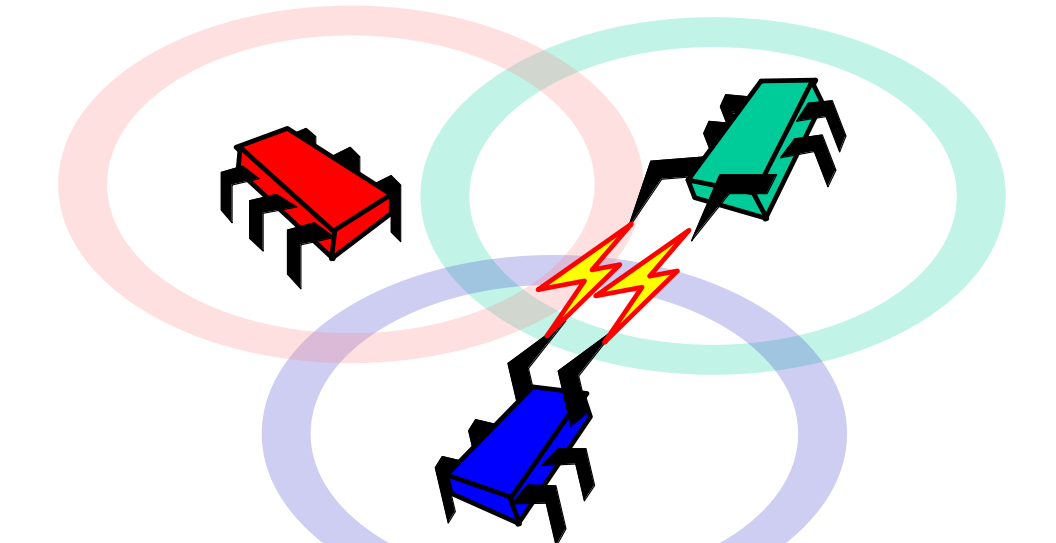
\includegraphics[width=0.5\textwidth]{./pics/consensus/cons2.png}
\end{center}

\end{frame}

\begin{frame}[noframenumbering]{They agree on some input}

\begin{center}
  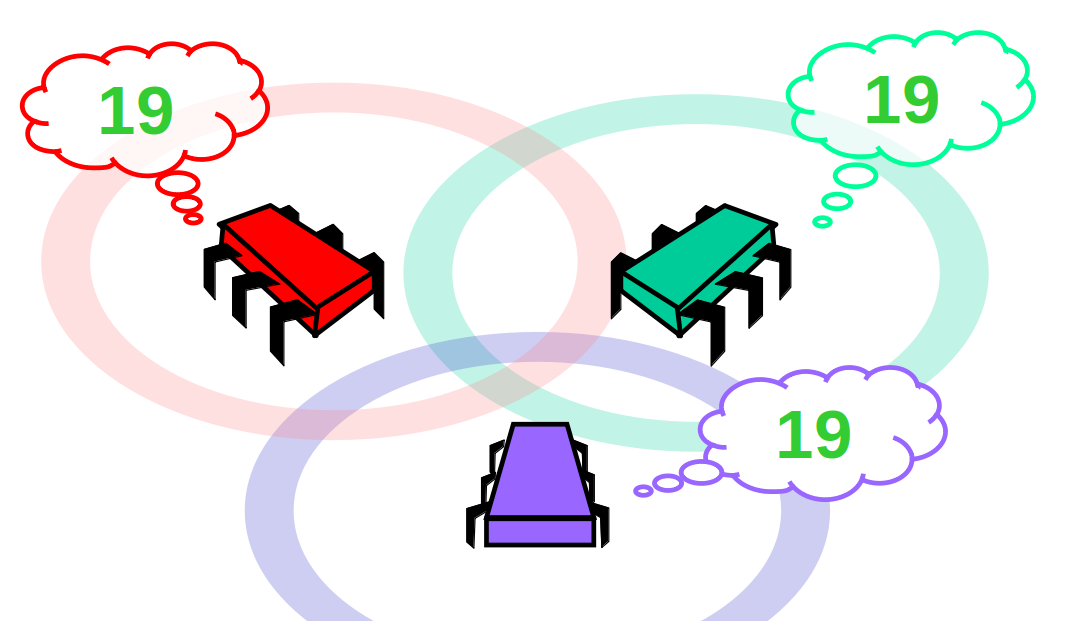
\includegraphics[width=0.5\textwidth]{./pics/consensus/cons3.png}
\end{center}
\end{frame}


\begin{frame}{Consensus}

\begin{itemize}
  \item \textbf{Consistent}: all threads decide the same value
  \item \textbf{Valid}: the common decision value is some thread's input
\end{itemize}

\pause

\begin{theorem}
  There is no wait-free implementation of n-thread consensus from read-write registers
\end{theorem}

\pause

Implication:
\begin{itemize}
  \item Asynchronous computability different from Turing computability
\end{itemize}

\pause

Read-write registers formalized in terms of safe/regular/atomic concurrent objects.

\pause

Theorem could be adapted to:

\begin{itemize}
  \item Registers
  \item Message-passing
  \item Carrier pigeons
  \item Any kind of asynchronous computation
\end{itemize}

\end{frame}


\begin{frame}{Consensus: why?}

\begin{itemize}
  \item \textbf{Consistent}: all threads decide the same value
  \item \textbf{Valid}: the common decision value is some thread's input
\end{itemize}

\begin{theorem}
  There is no wait-free implementation of n-thread consensus from read-write registers
\end{theorem}

\pause
Theorem helps to prove fun stuff, e.g. 
\begin{itemize}
  \item it is impossible to implement a two-dequeuer wait-free FIFO queue
  \item from read/write memory
\end{itemize}

\pause

Let's classify all concurrent objects by their "synchronization power"

\end{frame}

\begin{frame}{Consensus number}

An object \textbf{X} has \textit{consensus number} \textbf{n}
\begin{itemize}
  \item If it can be used to solve \textbf{n}-thread consensus
  \begin{itemize}
    \item Take any number of instances of \textbf{X} 
    \item together with atomic read/write registers
    \item and implement \textbf{n}-thread consensus
  \end{itemize}
  \item But not \textbf{(n+1)}-thread consensus
\end{itemize}

\pause

\begin{theorem}
  Atomic read/write registers have consensus number 1
\end{theorem}

Atomic registers cannot implement multiple assignment
\begin{itemize}
  \item Single write/multi read OK
  \item Multi write/multi read impossible
\end{itemize}

\end{frame}


\begin{frame}{Consensus number}

\begin{theorem}
  Atomic read/write registers have consensus number 1
\end{theorem}

Atomic registers cannot implement \only<2->{\textbf{wait-free}} multiple assignment
\begin{itemize}
  \item Single write/multi read OK
  \item Multi write/multi read impossible
\end{itemize}

\pause
\pause

\begin{theorem}
Multi-dequeuer FIFO queues have consensus number at least 2
\end{theorem}

Atomic registers cannot implement highly concurrent wait-free FIFO
\begin{itemize}
  \item it is impossible to implement a two-dequeuer wait-free FIFO queue
  \item from read/write memory
\end{itemize}

\end{frame}

\begin{frame}{Consensus numbers measure synchronization power}

\begin{theorem}
\begin{itemize}
  \item If you can implement \textbf{X} from \textbf{Y}
  \item And \textbf{X} has consensus number \textbf{c}
  \item Then \textbf{Y} has consensus number at least \textbf{c}
\end{itemize}
\end{theorem}

\pause

Registers have consensus number \textbf{1}

\pause

There are practically interesting problems that require higher consensus number

\pause

What should we do next?

\end{frame}

% \subsection{Atomic registers}
% 
% 
% \begin{frame}{Uni and bivalent states, critical state}
% 
% Theorem 
% There is no wait-free implementation of n-thread consensus from read-write registers
% Implication
% Asynchronous computability different from Turing computability
% 
% provibg easy case 38 - 91
% 
% \end{frame}
% 
% \begin{frame}{Atomic regs consensus 1}
% 
% Proof
% \end{frame}
% 
% 
% \begin{frame}{Astonishing practical result}
% 
% super-duper atomic read writes are NOT enough to impl cool lock-free/wait-free data structures
% 
% but what we could do fix fix limits 
 % - (2 threads? 3threads?)
 % - several atomic assignment?
% 
% we need something more strong (and hw engineers need to provide it)
 % - but which operations do we need?
% \end{frame}
% 
% 
% 
% \begin{frame}{Consensus for atomic registers: summary}
% 
% An object X has consensus number n
% If it can be used to solve n-thread consensus
% Take any number of instances of X 
% together with atomic read/write registers
% and implement n-thread consensus
% But not (n+1)-thread consensus
% 
% Theorem
% Atomic read/write registers have consensus number 1
% Theorem
% Multi-dequeuer FIFO queues have consensus number at least 2
% 
% \end{frame}
% 
% 
% \begin{frame}{Interesting facts: theory, no proof}
% 
% FIFO consensus
% (m, n) assignment consensus
% 
% TODO: show how to prove impossibility of mukti-write/multi-read using consusnsus!
% 
% 
% \end{frame}
% 
% 
% \subsection{Read-Modify-Write Operations (Common2)}
% 
% \begin{frame}{Interesting facts: hw, no proof}
% 
% Common2 ops, consensus number is exaclty 2, page 115 informal explanation
% 
% Conclusion: h/w getAndIncrement is not enough for consensus, we need something more elaborate
% 
% Remark: reminder that consensus is about wait freedom, you could develop a blocking mutex on getAndIncrement or some other stuff which is al least obstruction-free
% 
% \end{frame}
% 
% 
% \subsection{CompareAndSet}
% 
% \begin{frame}{CompareAndSwap CompareAndSet CompareAndExchange}
% 
% we have definition mess
% 
% java util concurrent
% c++
% papers/books
% 
% and variations of ret value, but they are trivially equivalent (theoretically, not practically TODO: JDK fro mshipilev about canhe beh, LEc-TODO)
% 
% 
% !!! CAS is infinirte consensus number
% 
% h/w enginers are relaxed now
% 
% \end{frame}


\section{Summary}

\begin{frame}{Summary}

Progress conditions
\begin{itemize}
  \item Dependent progress: Deadlock-freedom, Starvation-freedom
  \item Non-blocking progress: Lock-freedom, Wait-freedom
  \item Dependent non-blocking progress: Obstruction-freedom
\end{itemize}

Register design space
\begin{itemize}
  \item Capacity, Concurrency (SRSW, MRMW, MRMR), Consistency (safe, regular, atomic)
  \item Atomic snapshot
\end{itemize}

Wait-free constructions using
\begin{itemize}
  \item Timestamps, Helping/Cooperation, Decomposition 
\end{itemize}

New problems specific to non-blocking designs
\begin{itemize}
  \item Global clock, ABA
\end{itemize}

Consensus number as a tool to formalize relative synchronization power

% 
% we tried to assess different definitions and progress guarantees
% 
% but major focus was on wait-freedom
% because it is theoretically intersting and allows to "push the limits"
% 
% in reality we see that
% locking (no progress), obstr-free/lock-free/wait-free
% are growing complecxity and (usually) decresing performance (throughput) and even latency (because real world not only about upper bound but also about 99 percentile)
% 
% so do not mix theory and practice
% 
% 
% however all the key ideas: snapshotting, multi-value constructions, helping, re-check for clean view, RMW2 and CAS are all useful tools for reading/writing concurrent protocols
% 
% Further reading: uniersal consensu, book as a whole
% 
% more sophisticated and useful:
% distributed systems (building protocols form weaker primitevs -- no deliverey guarantee, no order guarantee), still need consensus:
  % devops/kubernetes/lxc
  % load balancing
  % datagrids
  % supercomputer data topology
  % ...

\end{frame}

\begin{frame}{Summary: homework}

\begin{homeworkcritical}
  \textbf{Easy}. Prove that Regular MRSW Integer construction is correct and wait-free.
  Use Section 4.2.3 "A Regular M-Valued MRSW Register"
\end{homeworkcritical}

\begin{homeworkcritical}
  \textbf{Medium}.
  \begin{itemize}      
    \item  Prove that "Simple snapshot" \ algorithm is correct, wait-free for \texttt{update()} and obstruction-free for \texttt{scan()}.
           Use Section 4.3.1 "An Obstruction-Free Snapshot".
    \item \textbf{Note:} algorithm uses stamped values, be ready to explain how it works in wait-free setting
  \end{itemize}
\end{homeworkcritical}

\begin{homeworkcritical}
  \textbf{Hard}. Solve exercise 41 from Section 4.5.
\end{homeworkcritical}

\end{frame}

\end{document}
